\documentclass[slidestop,compress,mathserif]{beamer}

%%% To get handouts:
%\documentclass[11pt,containsverbatim,handout]{beamer}
%% include when making handouts
%\usepackage{pgfpages}
%\pgfpagesuselayout{4 on 1}[letterpaper,landscape,border shrink=5mm]

%%% To get rid of solutions on handouts:
\newcommand{\soln}[1]{\textit{#1}}				% For slides
%\newcommand{\soln}[1]{ }	% For handouts

\newcommand{\solnGr}[1]{#1}
%\newcommand{\solnGr}{ }

\usetheme{metropolis}

%%%%%%%%%%%%%%%%
% Packages
%%%%%%%%%%%%%%%%

\usepackage{geometry}
\usepackage{graphicx}
\usepackage{amssymb}
%\usepackage{cancel}
\usepackage{epstopdf}
\usepackage{amsmath}  	% this permits text in eqnarray among other benefits
\usepackage{url}		% produces hyperlinks
\usepackage{hyperref}	% allows for color usage in tables
\usepackage[english]{babel}
\usepackage[latin1]{inputenc}
\usepackage{colortbl}	% allows for color usage in tables
\usepackage{multirow}	% allows for rows that span multiple rows in tables
\usepackage{color}		% this package has a variety of color options
\usepackage{pgf}
\usepackage{calc}
\usepackage{ulem}
\usepackage{multicol}
\usepackage{textcomp}
\usepackage{txfonts}
\usepackage{listings}
\usepackage{tikz}
\usepackage{array}
\usepackage{wasysym}
\usepackage{fancyvrb}


%%%%%%%%%%%%%%%%
% Remove navigation symbols
%%%%%%%%%%%%%%%%

\setbeamertemplate{navigation symbols}{}

%%%%%%%%%%%%%%%%
% User defined colors
%%%%%%%%%%%%%%%%

\xdefinecolor{oiB}{rgb}{0.22,0.52,0.72}
\definecolor{oiG}{rgb}{.298,.447,.114}
\xdefinecolor{hlblue}{rgb}{0.051,0.65,1}
\xdefinecolor{gray}{rgb}{0.5, 0.5, 0.5}
\xdefinecolor{darkGray}{rgb}{0.3, 0.3, 0.3}
\xdefinecolor{darkerGray}{rgb}{0.2, 0.2, 0.2}
\xdefinecolor{rubineRed}{rgb}{0.89,0,0.30}
\xdefinecolor{irishGreen}{rgb}{0,0.60,0}	
\definecolor{lightGreen}{rgb}{0.387,0.581,0.148} 

%%%%%%%%%%%%%%%%
% Template colors
%%%%%%%%%%%%%%%%

%\setbeamercolor*{palette primary}{fg=white,bg= oiB!80!black!90}
%\setbeamercolor*{palette secondary}{fg=black,bg= oiB!80!black}
%\setbeamercolor*{palette tertiary}{fg=white,bg= oiB!80!black!80}
%\setbeamercolor*{palette quaternary}{fg=white,bg= oiB}
%\setbeamercolor{structure}{fg= oiB}
%\setbeamercolor{frametitle}{bg= oiB!90}
%\setbeamertemplate{blocks}[shadow=false]
%\setbeamersize{text margin left=2em,text margin right=2em}

%\setbeamercolor{code body}{bg=gray!20!white!80,fg=black}


%%%%%%%%%%%%%%%%
% Get rid of fancy enumerated list bullets
%%%%%%%%%%%%%%%%

%\setbeamertemplate{enumerate items}[default]

%%%%%%%%%%%%%%%%
% Custom commands
%%%%%%%%%%%%%%%%

% degree
\newcommand{\degree}{\ensuremath{^\circ}}

% cite
\newcommand{\ct}[1]{
\vfill
{\tiny #1}}

% Note
\newcommand{\Note}[1]{
\rule{2.5cm}{0.25pt} \\ \textit{\footnotesize{\textcolor{rubineRed}{Note:} \textcolor{darkerGray}{#1}}}}

% Remember
\newcommand{\Remember}[1]{\textit{\scriptsize{\textcolor{orange}{Remember:} #1}}}

% expected counts
\newcommand{\ex}[1]{\textit{\textcolor{blue}{#1}}}

% red
\newcommand{\red}[1]{\textit{\textcolor{rubineRed}{#1}}}

% pink
\newcommand{\pink}[1]{\textit{\textcolor{rubineRed!90!white!50}{#1}}}

% green
\newcommand{\green}[1]{\textit{\textcolor{irishGreen}{#1}}}

% orange
\newcommand{\orange}[1]{\textit{\textcolor{orange}{#1}}}

% links: webURL, webLin, appLink
\newcommand{\webURL}[1]{\urlstyle{same}{ \textit{\textcolor{darkGray}{\url{#1}}}}}
\newcommand{\webLink}[2]{\href{#1}{\textcolor{darkGray}{{#2}}}}
\newcommand{\appLink}[2]{\href{#1}{\textcolor{white}{{#2}}}}

% mail
\newcommand{\mail}[1]{\href{mailto:#1}{\textit{\textcolor{darkGray}{#1}}}}

% highlighting: hl, hlGr, mathhl
\newcommand{\hl}[1]{\textit{\textcolor{hlblue}{#1}}}
\newcommand{\hlGr}[1]{\textit{\textcolor{lightGreen}{#1}}}
\newcommand{\mathhl}[1]{\textcolor{hlblue}{\ensuremath{#1}}}

% two col: two columns
\newenvironment{twocol}[4]{
\begin{columns}[c]
\column{#1\textwidth}
#3
\column{#2\textwidth}
#4
\end{columns}
}

% slot (for probability calculations)
\newenvironment{slot}[2]{
\begin{array}{c} 
\underline{#1} \\ 
#2
\end{array}
}

% pr: left and right parentheses
\newcommand{\pr}[1]{
\left( #1 \right)
}

% solnMult: solutions for practice questions

\newcommand{\solnMult}[1]{
\item[] \vspace{-0.59cm}
\only<1>{\item #1}
\soln{\only<2->{\item \orange{#1}}}
}

% cancel
\newcommand{\cancel}[1]{%
    \tikz[baseline=(tocancel.base)]{
        \node[inner sep=0pt,outer sep=0pt] (tocancel) {#1};
        \draw[red, line width=0.5mm] (tocancel.south west) -- (tocancel.north east);
    }%
}

% removepagenumbers
\newcommand{\removepagenumbers}{% 
  \setbeamertemplate{footline}{}
}

%%%%%%%%%%%%%%%%
% Custom boxes
%%%%%%%%%%%%%%%%

% app: application exercise

\setbeamercolor{app body}{fg=oiG}

\newcommand{\app}[1]{
\begin{beamerboxesrounded}[shadow = false, lower = app body]{}
#1
\end{beamerboxesrounded}
}

% dq: discussion question

\setbeamercolor{disc ques body}{fg=oiB}

\newcommand{\dq}[1]{
\begin{beamerboxesrounded}[shadow = false, lower = disc ques body]{}
#1
\end{beamerboxesrounded}
}

% pq: practice question

\setbeamercolor{prac ques body}{fg=oiB}

\newcommand{\pq}[1]{
\begin{beamerboxesrounded}[shadow = false, lower = prac ques body]{}
#1
\end{beamerboxesrounded}
}

% formula

\setbeamercolor{formula body}{fg=oiB!55!black!95}

\newcommand{\formula}[1]{
\begin{beamerboxesrounded}[shadow = false, lower = formula body]{}
#1
\end{beamerboxesrounded}
}


%%%%%%%%%%%%%%%%
% Change margin
%%%%%%%%%%%%%%%%

\newenvironment{changemargin}[2]{%
\begin{list}{}{%
\setlength{\topsep}{0pt}%
\setlength{\leftmargin}{#1}%
\setlength{\rightmargin}{#2}%
\setlength{\listparindent}{\parindent}%
\setlength{\itemindent}{\parindent}%
\setlength{\parsep}{\parskip}%
}%
\item}{\end{list}}

%%%%%%%%%%%%%%%%
% Footnote
%%%%%%%%%%%%%%%%

\long\def\symbolfootnote[#1]#2{\begingroup%
\def\thefootnote{\fnsymbol{footnote}}\footnote[#1]{#2}\endgroup}

%%%%%%%%%%%%%%%%
% Commands from the book
%%%%%%%%%%%%%%%%

\newenvironment{data}[1]{\texttt{#1}}{}
\newenvironment{var}[1]{\texttt{#1}}{}
\newenvironment{resp}[1]{\texttt{#1}}{}

%%%%%%%%%%%%%%%%
% Graphics
%%%%%%%%%%%%%%%%

\DeclareGraphicsRule{.tif}{png}{.png}{`convert #1 `dirname #1`/`basename #1 .tif`.png}

%%%%%%%%%%%%%%%%%%%%%

\title[Chp 7: Intro. to linear regression]{Chapter 7: Introduction to linear regression}
\author{OpenIntro Statistics, 2nd Edition}
\date{}
\institute{}

%%%%%%%%%%%%%%%%%%%%%

\begin{document}

%%%%%%%%%%%%%%%%%%%%%

% Title Page

\begin{frame}[plain]

\titlepage

\end{frame}

%%%%%%%%%%%%%%%%%%%%%%%%%%%%%%%%%%%%

%%%%%%%%%%%%%%%%%%%%%%%%%%%%%%%%%%%%

\section{Line fitting, residuals, and correlation}

%%%%%%%%%%%%%%%%%%%%%%%%%%%%%%%%%%%%

\begin{frame}
\frametitle{Modeling numerical variables}

In this unit we will learn to quantify the relationship between two numerical variables, as well as modeling numerical response variables using a numerical or categorical explanatory variable.

\end{frame}

%%%%%%%%%%%%%%%%%%%%%%%%%%%%%%%%%%%%

\begin{frame}
\frametitle{Poverty vs. HS graduate rate}

The \hl{scatterplot} below shows the relationship between HS graduate rate in all 50 US states and DC and the \% of residents who live below the poverty line {\small (income below \$23,050 for a family of 4 in 2012)}.

\twocol{0.55}{0.45}{
\begin{center}
\includegraphics[width=\textwidth]{7-1_linefit_res_corr/figures/poverty/poverty_hsgrad}
\end{center}
}
{
\dq{Response variable?}
\pause
\soln{\% in poverty}
\pause
\dq{Explanatory variable?}
\pause
\soln{\% HS grad}
\pause
\dq{Relationship?}
\pause
\soln{linear, negative, moderately strong}
}

\end{frame}

%%%%%%%%%%%%%%%%%%%%%%%%%%%%%%%%%%%

\begin{frame}
\frametitle{Quantifying the relationship}

\begin{itemize}

\item \hl{Correlation} describes the strength of the \orange{linear} association between two variables.

\pause

\item It takes values between -1 (perfect negative) and +1 (perfect positive).

\pause

\item A value of 0 indicates no linear association.

\end{itemize}

\end{frame}

%%%%%%%%%%%%%%%%%%%%%%%%%%%%%%%%%%%

\begin{frame}
\frametitle{Guessing the correlation}

\pq{Which of the following is the best guess for the correlation between \% in poverty and \% HS grad?}
\twocol{0.4}{0.6}
{
\begin{enumerate}[(a)]
\item 0.6
\solnMult{-0.75}
\item -0.1
\item 0.02
\item -1.5
\end{enumerate}
}
{
\begin{center}
\includegraphics[width=\textwidth]{7-1_linefit_res_corr/figures/poverty/poverty_hsgrad_line}
\end{center}
}

\end{frame}

%%%%%%%%%%%%%%%%%%%%%%%%%%%%%%%%%%

\begin{frame}
\frametitle{Guessing the correlation}

\pq{Which of the following is the best guess for the correlation between \%~in~poverty and \% HS grad?}

\twocol{0.4}{0.6}
{
\begin{enumerate}[(a)]
\item 0.1
\item -0.6
\item -0.4
\item 0.9
\solnMult{0.5}
\end{enumerate}
}
{
\begin{center}
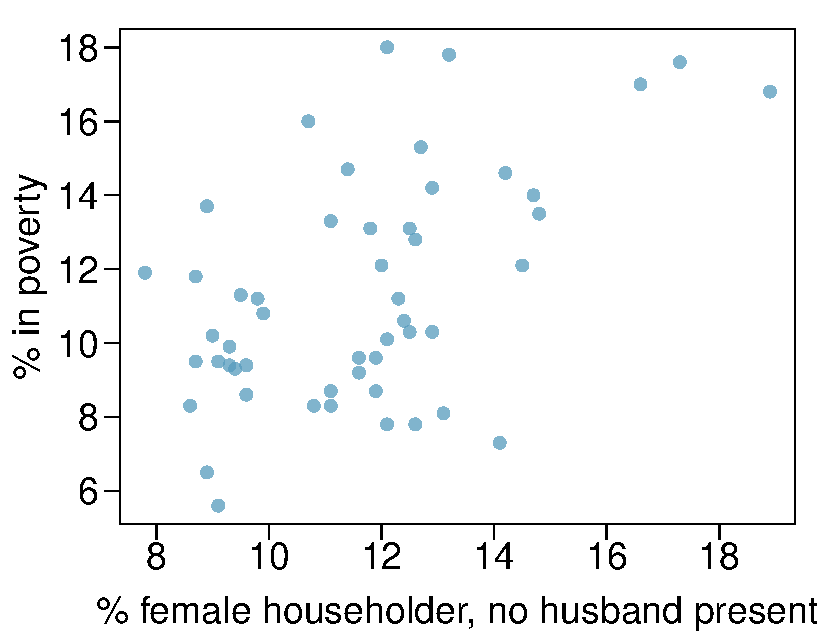
\includegraphics[width=\textwidth]{7-1_linefit_res_corr/figures/poverty/poverty_nohusband}
\end{center}
}

\end{frame}

%%%%%%%%%%%%%%%%%%%%%%%%%%%%%%%%%%

\begin{frame}
\frametitle{Assessing the correlation}

\pq{Which of the following is has the strongest correlation, i.e. correlation coefficient closest to +1 or -1?}

\twocol{0.8}{0.2}
{
\begin{center}
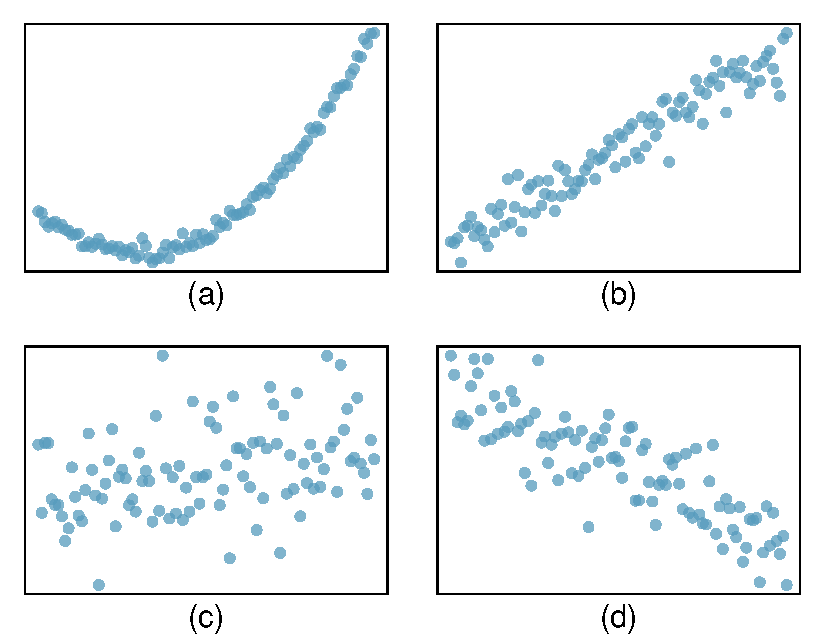
\includegraphics[width=0.75\textwidth]{7-1_linefit_res_corr/figures/cor/cor}
\end{center}
}
{
\soln{\only<2>{\orange{
(b) $\rightarrow$ correlation means \underline{linear} association
}}}
}

\end{frame}

\section{Fitting a line by least squares regression}

%%%%%%%%%%%%%%%%%%%%%%%%%%%%%%%%%%%%

\subsection{Eyeballing the line}

%%%%%%%%%%%%%%%%%%%%%%%%%%%%%%%%%%%

\begin{frame}
\frametitle{Eyeballing the line}

\twocol{0.3}{0.7}
{
\pq{Which of the following appears to be the line that best fits the linear relationship between \% in poverty and \% HS grad? Choose one.}
\soln{\only<2>{\red{
(a)
}}}
}
{
\begin{center}
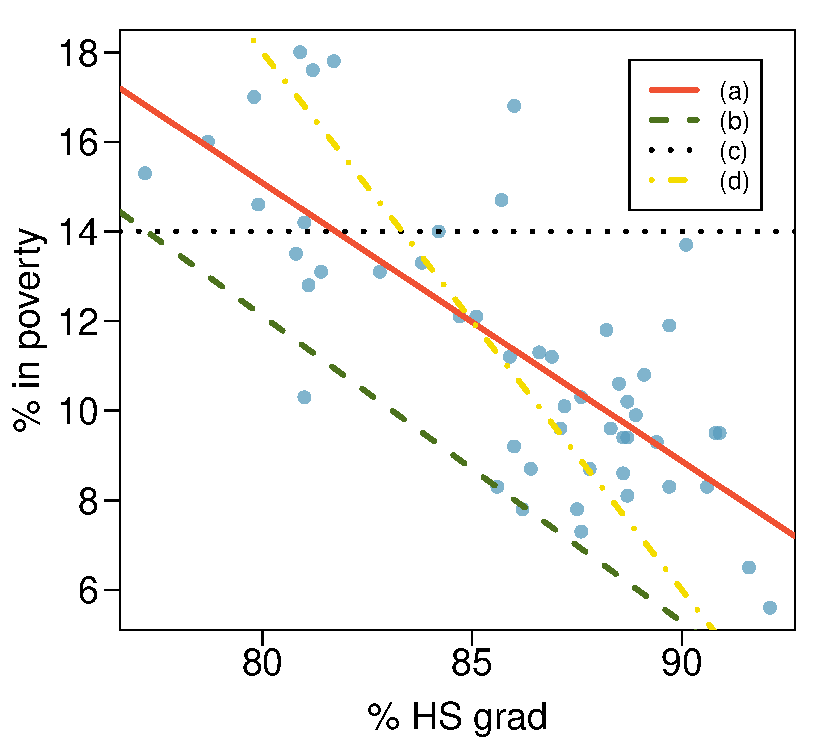
\includegraphics[width=\textwidth]{7-2_least_square_reg/figures/poverty/poverty_hsgrad_manylines}
\end{center}
}
\end{frame}

%%%%%%%%%%%%%%%%%%%%%%%%%%%%%%%%%%%

\subsection{Residuals}

%%%%%%%%%%%%%%%%%%%%%%%%%%%%%%%%%%%

\begin{frame}
\frametitle{Residuals}

\hl{Residuals} are the leftovers from the model fit: Data = Fit + Residual

\begin{center}
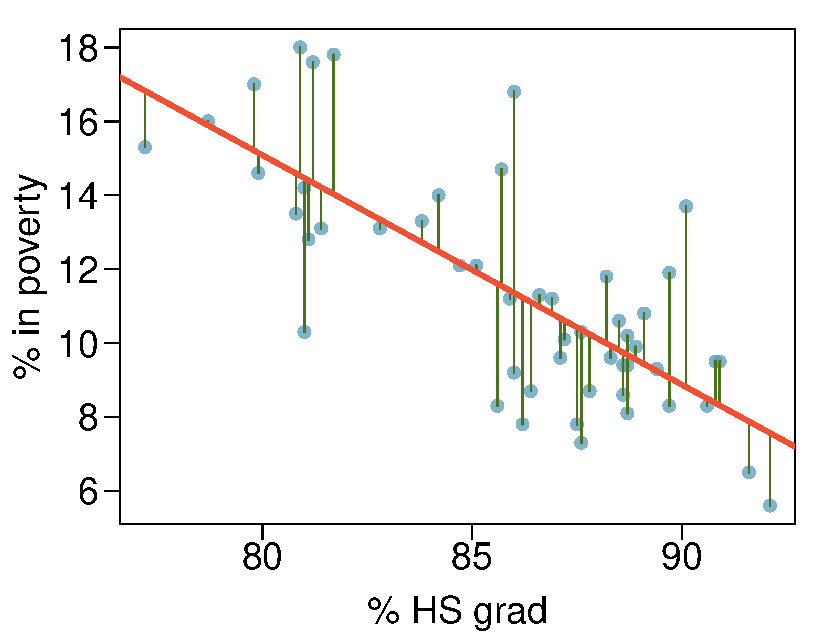
\includegraphics[width=0.8\textwidth]{7-2_least_square_reg/figures/poverty/poverty_hsgrad_res}
\end{center}

\end{frame}

%%%%%%%%%%%%%%%%%%%%%%%%%%%%%%%%%%

\begin{frame}
\frametitle{Residuals (cont.)}

\formula{Residual}{
Residual is the difference between the observed ($y_i$) and predicted $\hat{y}_i$. 
\[ e_i = y_i - \hat{y}_i \]
}
\vspace{-0.5cm}
\twocol{0.6}{0.4}
{
\begin{center}
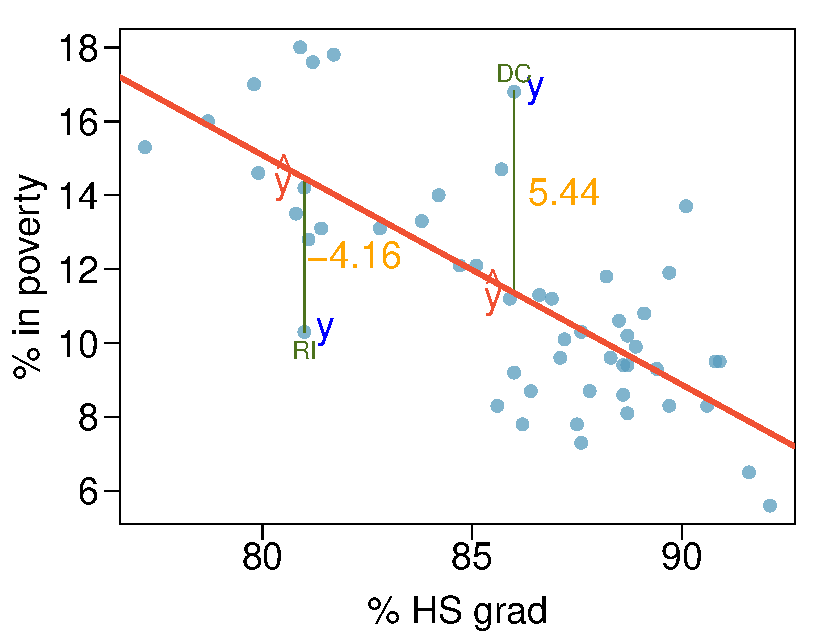
\includegraphics[width=\textwidth]{7-2_least_square_reg/figures/poverty/poverty_hsgrad_res_text}
\end{center}
}
{
\pause
\begin{itemize}
\item \% living in poverty in DC is 5.44\% more than predicted.
\pause
\item \% living in poverty in RI is 4.16\% less than predicted.
\end{itemize}
}


\end{frame}

%%%%%%%%%%%%%%%%%%%%%%%%%%%%%%%%%%

\subsection{Best line}

%%%%%%%%%%%%%%%%%%%%%%%%%%%%%%%%%%%

\begin{frame}
\frametitle{A measure for the best line}

\begin{itemize}

\item We want a line that has small residuals:
\pause
\begin{enumerate}
\item Option 1: Minimize the sum of magnitudes (absolute values) of residuals
\[ |e_1| + |e_2| + \cdots + |e_n| \]
\pause
\item Option 2: Minimize the sum of squared residuals -- \hl{least squares}
\[ e_1^2 + e_2^2 + \cdots + e_n^2 \]
\end{enumerate}

\pause

\item Why least squares?
\pause
\begin{enumerate}
\item Most commonly used
\pause
\item Easier to compute by hand and using software
\pause
\item In many applications, a residual twice as large as another is usually more than twice as bad
\end{enumerate}

\end{itemize}

\end{frame}

%%%%%%%%%%%%%%%%%%%%%%%%%%%%%%%%%%

\begin{frame}
\frametitle{The least squares line}

\[ \mathhl{ \hat{y} = \beta_0 + \beta_1 x } \]

\setlength{\unitlength}{0.75mm}
\begin{picture}(5,0)
\put(62.5,5){\vector(-2,-1){20}}
\put(18,-5){\red{predicted y}}
\end{picture}

\begin{picture}(5,0)
\put(70,10){\vector(-1,-1){15}}
\put(50,-10){\red{intercept}}
\end{picture}

\begin{picture}(5,0)
\put(80,15){\vector(1,-1){10}}
\put(90,0){\red{slope}}
\end{picture}

\begin{picture}(5,0)
\put(90,22.5){\vector(2,-1){20}}
\put(110,8){\red{explanatory variable}}
\end{picture}

\hl{Notation:}
\begin{itemize}

\item Intercept:
\begin{itemize}
\item Parameter: $\beta_0$ \\
\item Point estimate: $b_0$ \\
\end{itemize}

\item Slope:
\begin{itemize}
\item Parameter: $\beta_1$ \\
\item Point estimate: $b_1$ \\
\end{itemize}

\end{itemize}


\end{frame}

%%%%%%%%%%%%%%%%%%%%%%%%%%%%%%%%%%

\subsection{The least squares line}

%%%%%%%%%%%%%%%%%%%%%%%%%%%%%%%%%%%

\begin{frame}
\frametitle{Given...}

\twocol{0.5}{0.5}
{
\begin{center}
\includegraphics[width=\textwidth]{7-2_least_square_reg/figures/poverty/poverty_hsgrad}
\end{center}
}
{
\begin{tabular}{l r r}
\hline
		& \% HS grad		& \% in poverty \\
		& $(x)$			& $(y)$ \\
\hline
mean	& $\bar{x} = 86.01$	& $\bar{y} = 11.35$  \\
sd		& $s_x = 3.73$		& $s_y = 3.1$ \\
\hline
		& correlation		& $R = -0.75$ \\
\hline
\end{tabular}
}

\end{frame}

%%%%%%%%%%%%%%%%%%%%%%%%%%%%%%%%%%

\begin{frame}
\frametitle{Slope}

\formula{Slope}
{The slope of the regression can be calculated as 
\[ b_1 = \frac{s_y}{s_x} R \]
}

\pause

\hl{In context...}
\[ b_1 = \frac{3.1}{3.73} \times -0.75 = -0.62 \]

\pause
$\:$ \\
\hl{Interpretation} \\
For each additional \% point in HS graduate rate, we would expect the \% living in poverty to be lower on average by 0.62\% points.

\end{frame}

%%%%%%%%%%%%%%%%%%%%%%%%%%%%%%%%%%

\begin{frame}
\frametitle{Intercept}

\formula{Intercept}
{The intercept is where the regression line intersects the $y$-axis. The calculation of the intercept uses the fact the a regression line always passes through $(\bar{x},\bar{y})$.
\[ b_0 = \bar{y} - b_1 \bar{x} \]
}

\pause

\twocol{0.68}{0.32}
{
\begin{center}
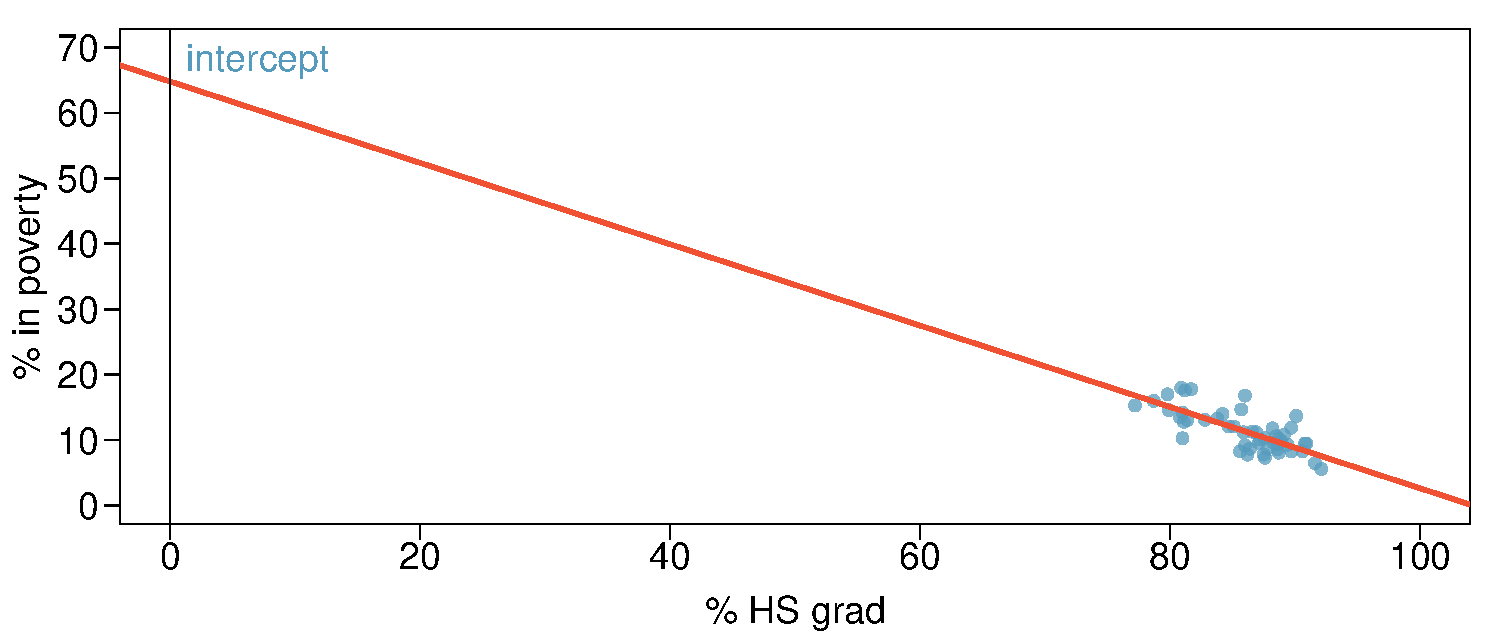
\includegraphics[width=\textwidth]{7-2_least_square_reg/figures/poverty/poverty_hsgrad_line_wide}
\end{center}
}
{
\pause
\begin{align*}
b_0 &= 11.35 - (-0.62) \times 86.01 \\
&= 64.68
\end{align*}
}

\end{frame}

%%%%%%%%%%%%%%%%%%%%%%%%%%%%%%%%%%

\begin{frame}
\frametitle{}

\pq{Which of the following is the correct interpretation of the intercept?}

\begin{enumerate}[(a)]
\item For each \% point increase in HS graduate rate, \% living in poverty is expected to increase on average by 64.68\%.
\item For each \% point decrease in HS graduate rate, \% living in poverty is expected to increase on average by 64.68\%.
\item Having no HS graduates leads to 64.68\% of residents living below the poverty line.
\solnMult{States with no HS graduates are expected on average to have 64.68\% of residents living below the poverty line.}
\item In states with no HS graduates \% living in poverty is expected to increase on average by 64.68\%.
\end{enumerate}

\end{frame}

%%%%%%%%%%%%%%%%%%%%%%%%%%%%%%%%%%%

\begin{frame}
\frametitle{More on the intercept}

Since there are no states in the dataset with no HS graduates, the intercept is of no interest, not very useful, and also not reliable since the predicted value of the intercept is so far from the bulk of the data.

\begin{center}
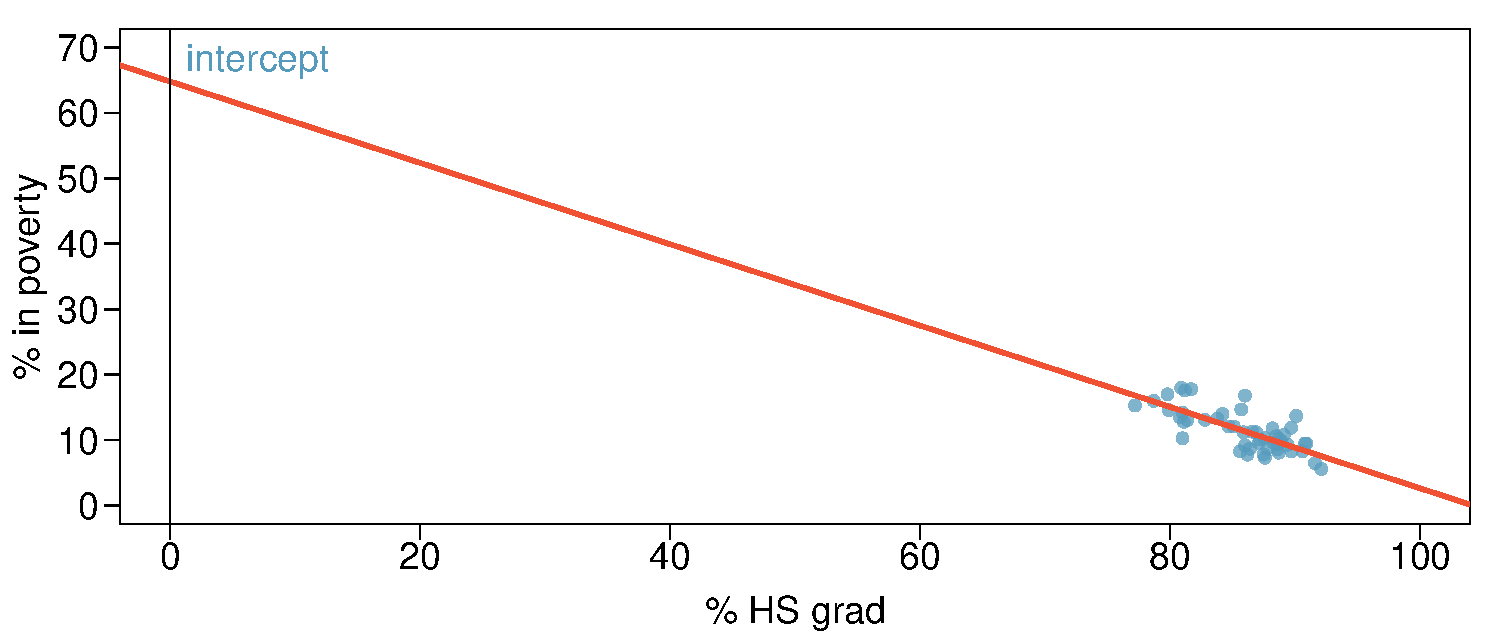
\includegraphics[width=\textwidth]{7-2_least_square_reg/figures/poverty/poverty_hsgrad_line_wide}
\end{center}

\end{frame}

%%%%%%%%%%%%%%%%%%%%%%%%%%%%%%%%%%

\begin{frame}
\frametitle{Regression line}

\[ \widehat{\%~in~poverty} = 64.68 - 0.62~\%~HS~grad \]

\begin{center}
\includegraphics[width=0.7\textwidth]{7-2_least_square_reg/figures/poverty/poverty_hsgrad_line}
\end{center}

\end{frame}

%%%%%%%%%%%%%%%%%%%%%%%%%%%%%%%%%%

\subsection{Recap: Interpreting the slope and the intercept}

%%%%%%%%%%%%%%%%%%%%%%%%%%%%%%%%%%%

\begin{frame}
\frametitle{Interpretation of slope and intercept}

\twocol{0.5}{0.5}{
\begin{itemize}

\item \hl{Intercept:} When {$x = 0$}, {$y$} is expected to equal {the intercept}. \\

$\:$ \\

\item \hl{Slope:} For each {unit} in {$x$}, {$y$} is expected to {increase / decrease} on average by {the slope}.

\end{itemize}
}
{
\begin{center}
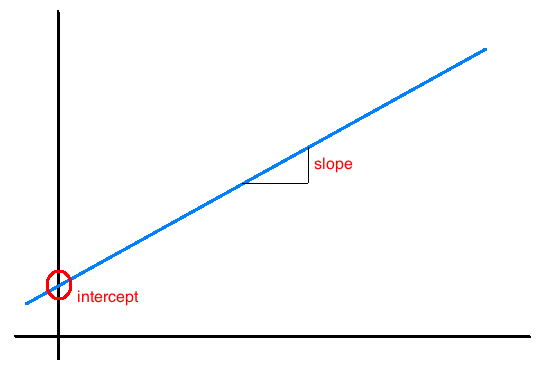
\includegraphics[width=\textwidth]{7-2_least_square_reg/figures/diagram}
\end{center}
}

\vspace{1cm}

\Note{These statements are not causal, unless the study is a randomized controlled experiment.}

\end{frame}


%%%%%%%%%%%%%%%%%%%%%%%%%%%%%%%%%%

\subsection{Prediction \& extrapolation}

%%%%%%%%%%%%%%%%%%%%%%%%%%%%%%%%%%


\begin{frame}
\frametitle{Prediction}

\begin{itemize}

\item Using the linear model to predict the value of the response variable for a given value of the explanatory variable is called \hl{prediction}, simply by plugging in the value of $x$ in the linear model equation.

\item There will be some uncertainty associated with the predicted value.

\end{itemize}

\begin{center}
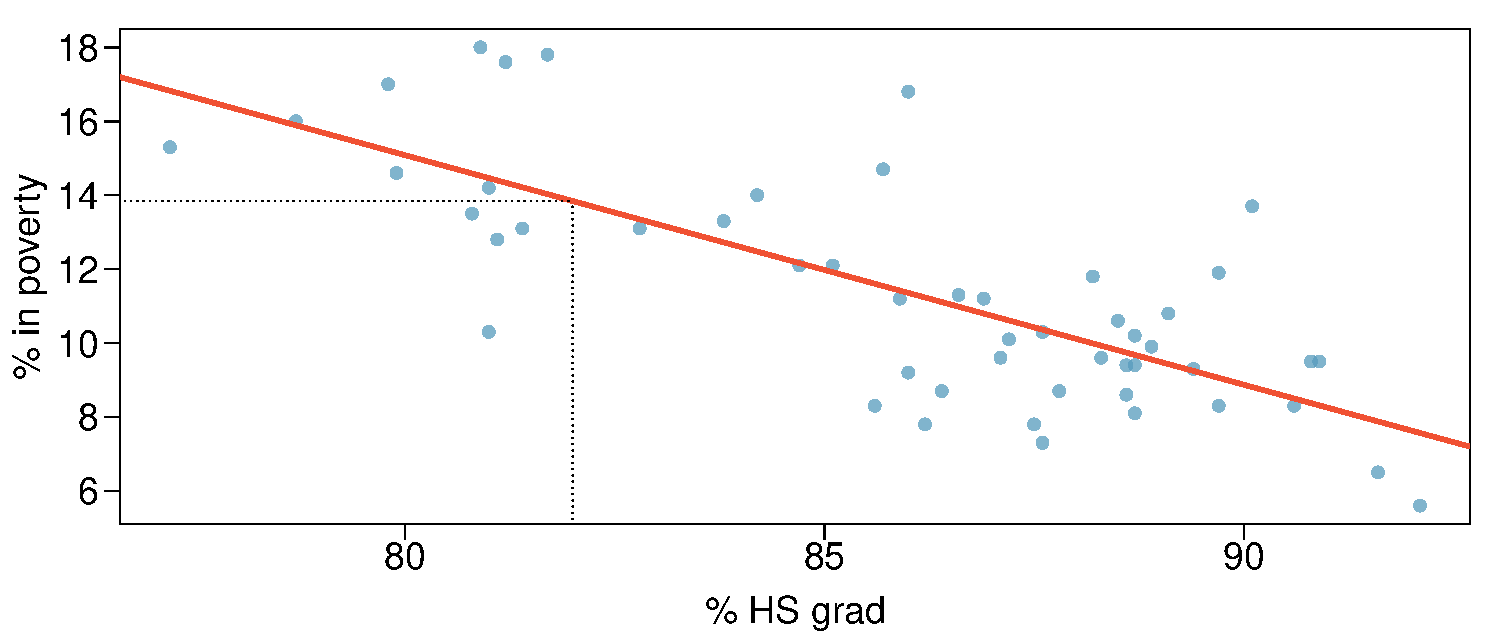
\includegraphics[width=0.9\textwidth]{7-2_least_square_reg/figures/poverty/poverty_hsgrad_pred}
\end{center}

\end{frame}

%%%%%%%%%%%%%%%%%%%%%%%%%%%%%%%%%%

\begin{frame}
\frametitle{Extrapolation}

\begin{itemize}

\item Applying a model estimate to values outside of the realm of the original data is called \hl{extrapolation}.

\item Sometimes the intercept might be an extrapolation.

\end{itemize}

\begin{center}
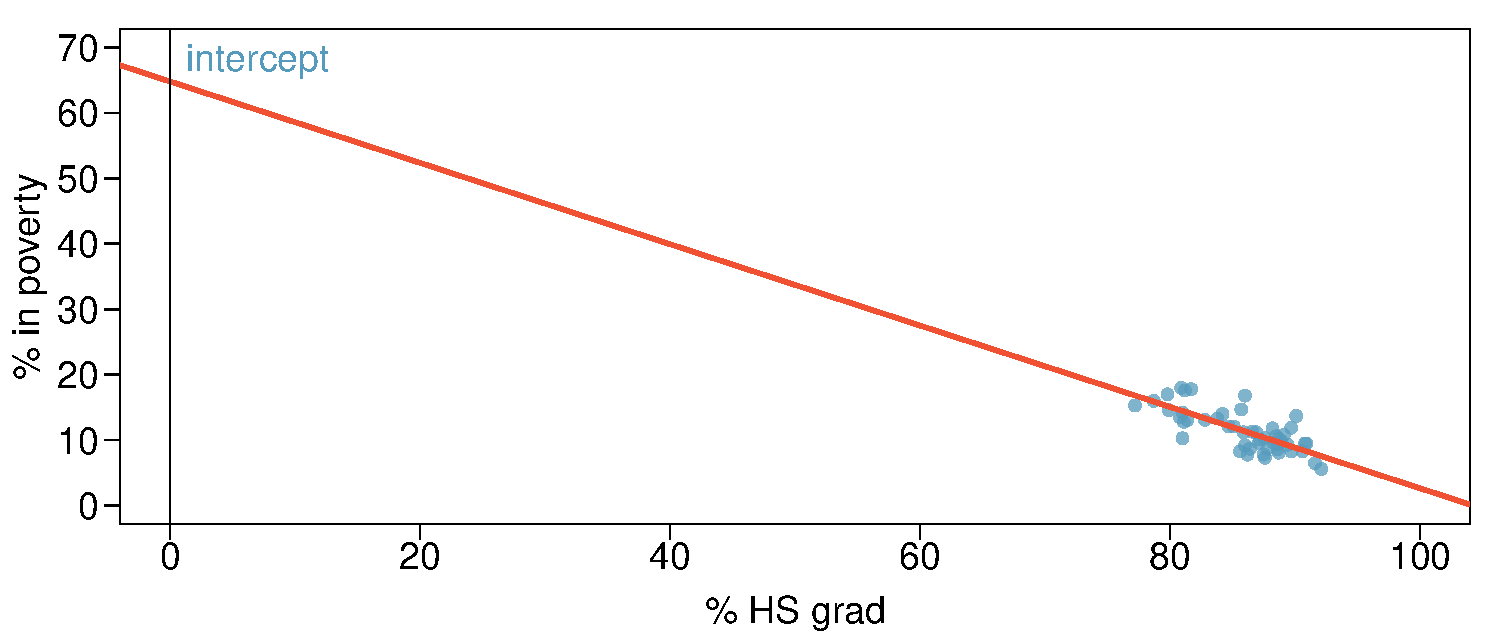
\includegraphics[width=\textwidth]{7-2_least_square_reg/figures/poverty/poverty_hsgrad_line_wide}
\end{center}

\end{frame}

%%%%%%%%%%%%%%%%%%%%%%%%%%%%%%%%%%

\begin{frame}
\frametitle{Examples of extrapolation}

\begin{center}
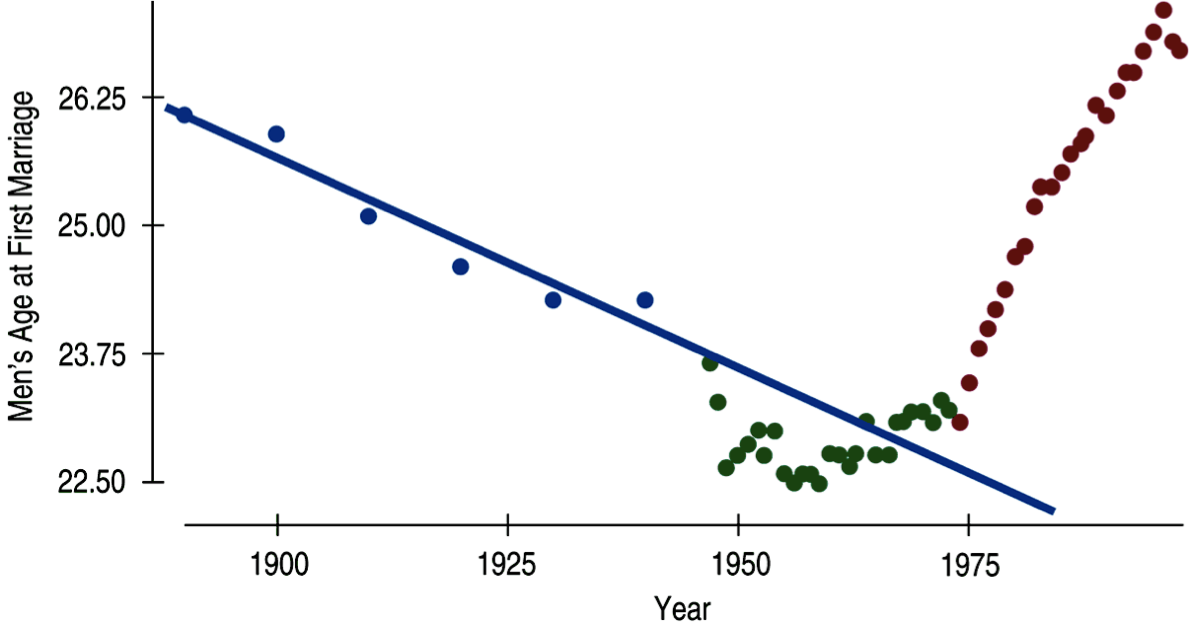
\includegraphics[width=\textwidth]{7-2_least_square_reg/figures/extrapolation}
\end{center}

\end{frame}

%%%%%%%%%%%%%%%%%%%%%%%%%%%%%%%%%%

\begin{frame}
\frametitle{Examples of extrapolation}

\begin{center}
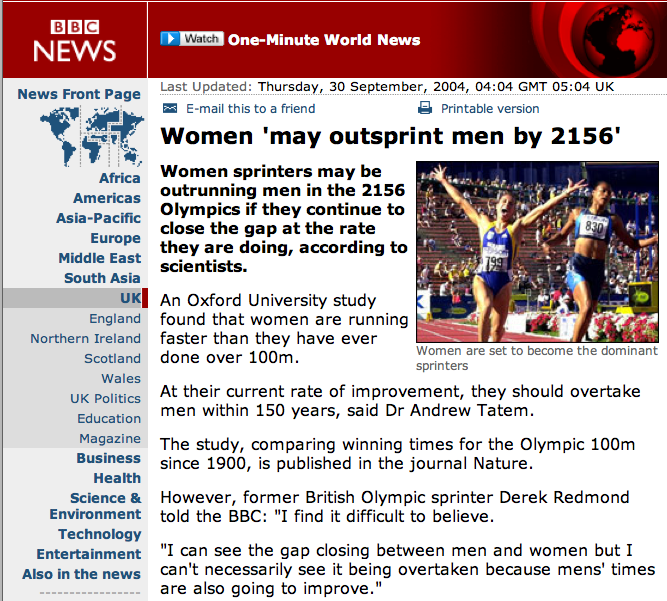
\includegraphics[width=0.7\textwidth]{7-2_least_square_reg/figures/womenOutsprintBBC}
\end{center}

\end{frame}

%%%%%%%%%%%%%%%%%%%%%%%%%%%%%%%%%%

\begin{frame}
\frametitle{Examples of extrapolation}

\begin{center}
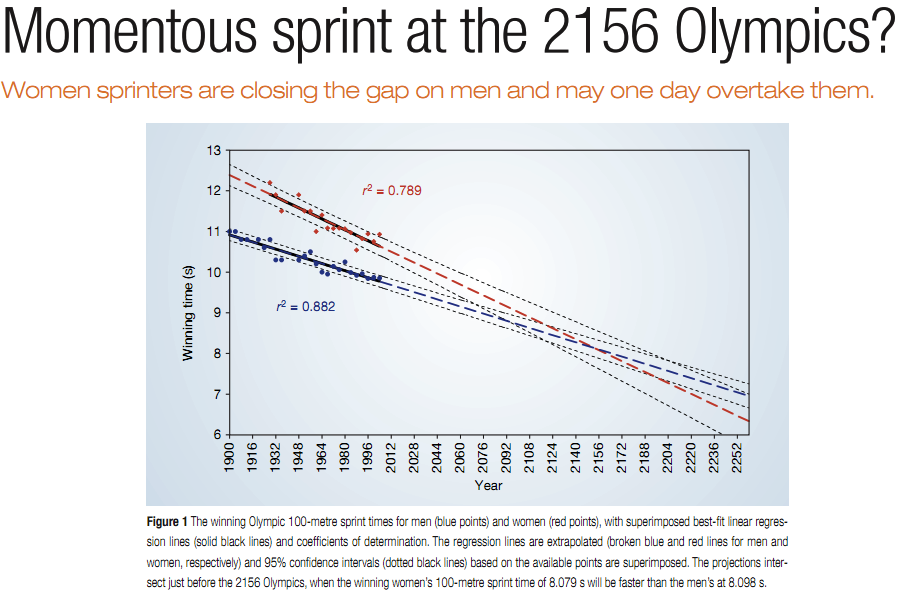
\includegraphics[width=\textwidth]{7-2_least_square_reg/figures/womenOutsprint}
\end{center}

\end{frame}

%%%%%%%%%%%%%%%%%%%%%%%%%%%%%%%%%%

\subsection{Conditions for the least squares line}

%%%%%%%%%%%%%%%%%%%%%%%%%%%%%%%%%%%

\begin{frame}
\frametitle{Conditions for the least squares line}

\begin{enumerate}

\item Linearity

\pause

\item Nearly normal residuals

\pause

\item Constant variability

\end{enumerate}

\end{frame}

%%%%%%%%%%%%%%%%%%%%%%%%%%%%%%%%%%

\begin{frame}
\frametitle{Conditions: (1) Linearity}

\begin{itemize}

\item The relationship between the explanatory and the response variable should be linear. 

\pause

\item Methods for fitting a model to non-linear relationships exist, but are beyond the scope of this class. If this topic is of interest, an \href{http://www.openintro.org/download.php?file=os2_extra_nonlinear_relationships&referrer=/stat/textbook.php}{Online Extra is available on openintro.org} covering new techniques.

\pause

\item Check using a scatterplot of the data, or a \hl{residuals plot}.

\end{itemize}

\begin{center}
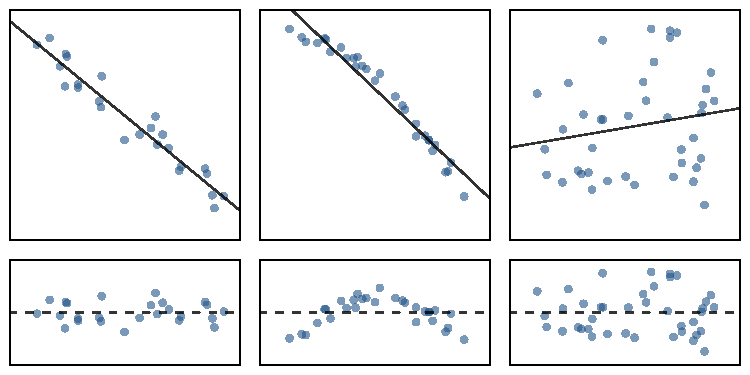
\includegraphics[width=0.7\textwidth]{7-2_least_square_reg/figures/sampleLinesAndResPlots/sampleLinesAndResPlots}
\end{center}

\end{frame}

%%%%%%%%%%%%%%%%%%%%%%%%%%%%%%%%%%

\begin{frame}
\frametitle{Anatomy of a residuals plot}

\twocol{0.5}{0.5}
{
\begin{center}
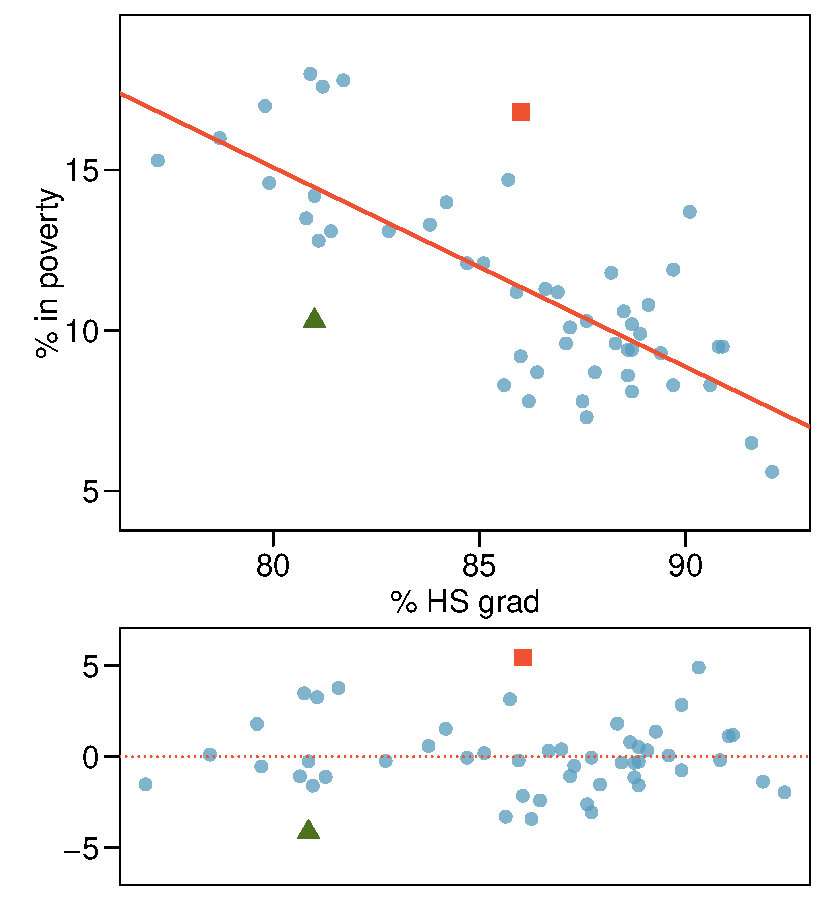
\includegraphics[width=\textwidth]{7-2_least_square_reg/figures/poverty/poverty_hsgrad_resplot}
\end{center}
}
{
\green{{\LARGE $\blacktriangle$}} \hl{RI:}
\begin{align*}
\%~HS~grad &= 81 \qquad \%~in~poverty = 10.3 \\
\widehat{\%~in~poverty} &= 64.68 - 0.62 * 81 = 14.46 \\
e &= \%~in~poverty - \widehat{\%~in~poverty} \\
&= 10.3 - 14.46 = \green{$-4.16$}
\end{align*}
$\:$
\pause
\textcolor{red}{{\Large $\blacksquare$}} \hl{DC:}
\begin{align*}
\%~HS~grad &= 86 \qquad \%~in~poverty = 16.8 \\
\widehat{\%~in~poverty} &= 64.68 - 0.62 * 86 = 11.36 \\
e &= \%~in~poverty - \widehat{\%~in~poverty} \\
&= 16.8 - 11.36 = \textcolor{red}{5.44}
\end{align*}
}

\end{frame}


%%%%%%%%%%%%%%%%%%%%%%%%%%%%%%%%%%

\begin{frame}
\frametitle{Conditions: (2) Nearly normal residuals}

\begin{itemize}

\item The residuals should be nearly normal.

\pause

\item This condition may not be satisfied when there are unusual observations that don't follow the trend of the rest of the data.

\pause

\item Check using a histogram or normal probability plot of residuals.

\end{itemize}

\begin{center}
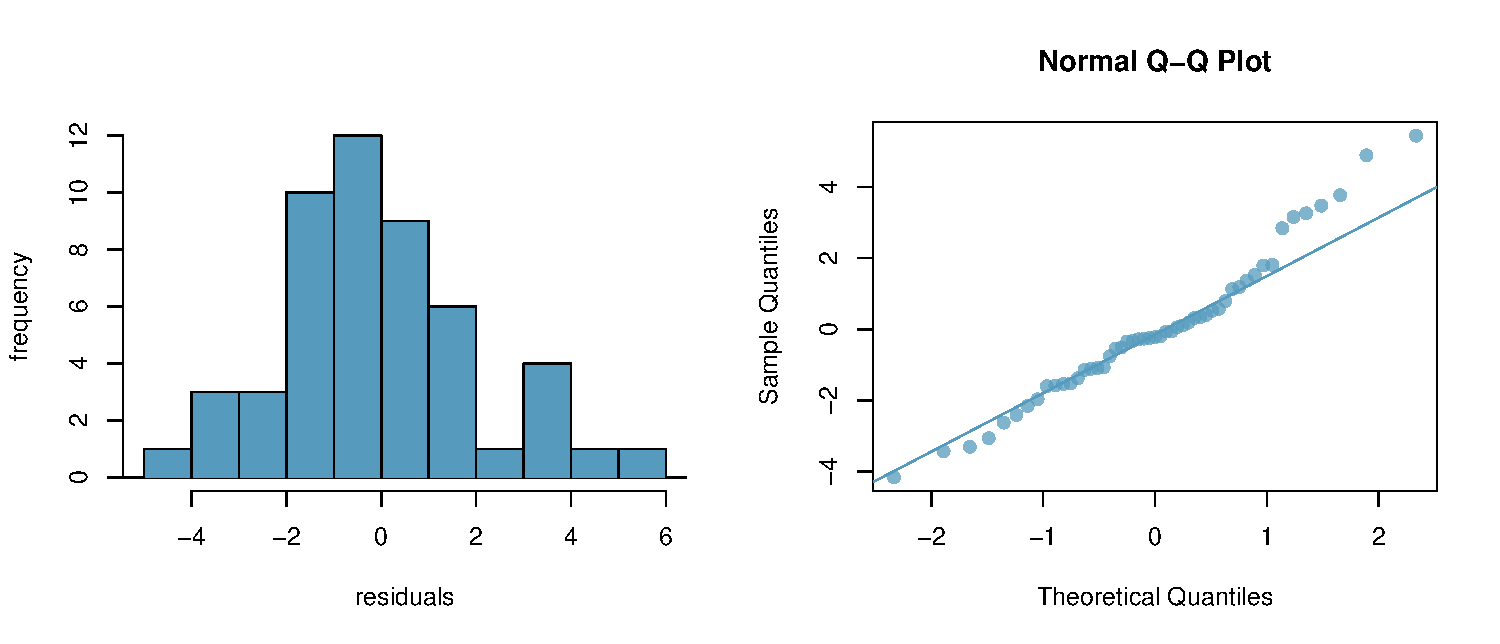
\includegraphics[width=\textwidth]{7-2_least_square_reg/figures/poverty/normal_res}
\end{center}

\end{frame}

%%%%%%%%%%%%%%%%%%%%%%%%%%%%%%%%%%

\begin{frame}
\frametitle{Conditions: (3) Constant variability}

\twocol{0.5}{0.5}
{
\begin{center}
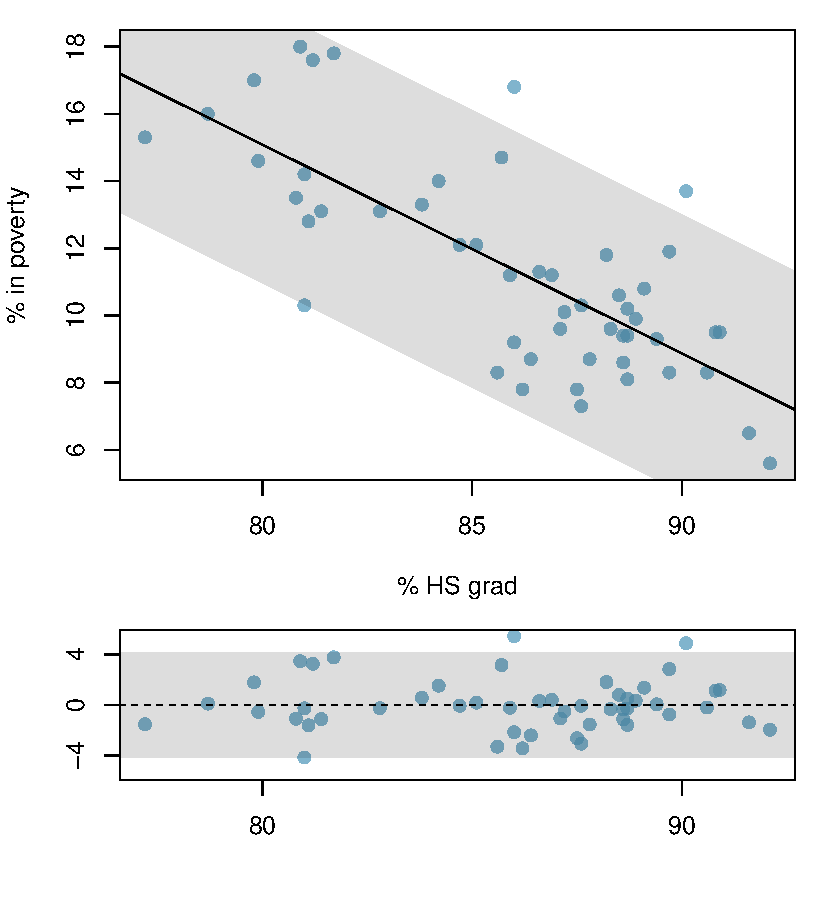
\includegraphics[width=\textwidth]{7-2_least_square_reg/figures/poverty/poverty_hsgrad_tube}
\end{center}
}
{
\begin{itemize}

\item The variability of points around the least squares line should be roughly constant.

\pause

\item This implies that the variability of residuals around the 0 line should be roughly constant as well.

\pause

\item Also called \hl{homoscedasticity}.

\pause

\item Check using a histogram or normal probability plot of residuals.

\end{itemize}
}


\end{frame}

%%%%%%%%%%%%%%%%%%%%%%%%%%%%%%%%%%

\begin{frame}
\frametitle{Checking conditions}

\twocol{0.5}{0.5}
{
\pq{What condition is this linear model obviously violating?}
\begin{enumerate}[(a)]
\item Constant variability
\solnMult{Linear relationship}
\item Normal residuals
\item No extreme outliers
\end{enumerate}
}
{
\begin{center}
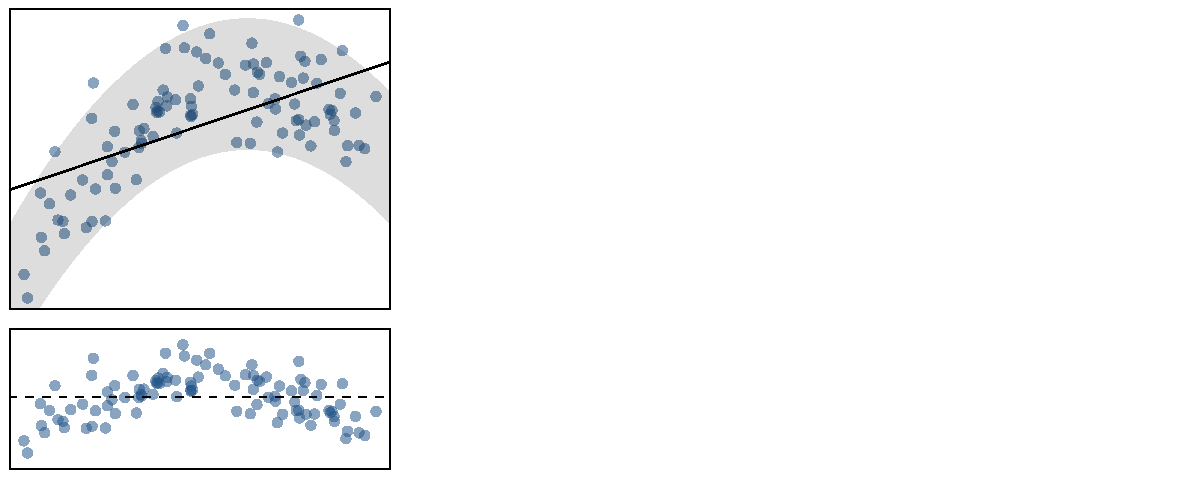
\includegraphics[width=\textwidth]{7-2_least_square_reg/figures/problems/nonlinear}
\end{center}
}

\end{frame}

%%%%%%%%%%%%%%%%%%%%%%%%%%%%%%%%%%

\begin{frame}
\frametitle{Checking conditions}

\twocol{0.5}{0.5}
{
\pq{What condition is this linear model obviously violating?}
\begin{enumerate}[(a)]
\solnMult{ Constant variability}
\item Linear relationship
\item Normal residuals
\item No extreme outliers
\end{enumerate}
}
{
\begin{center}
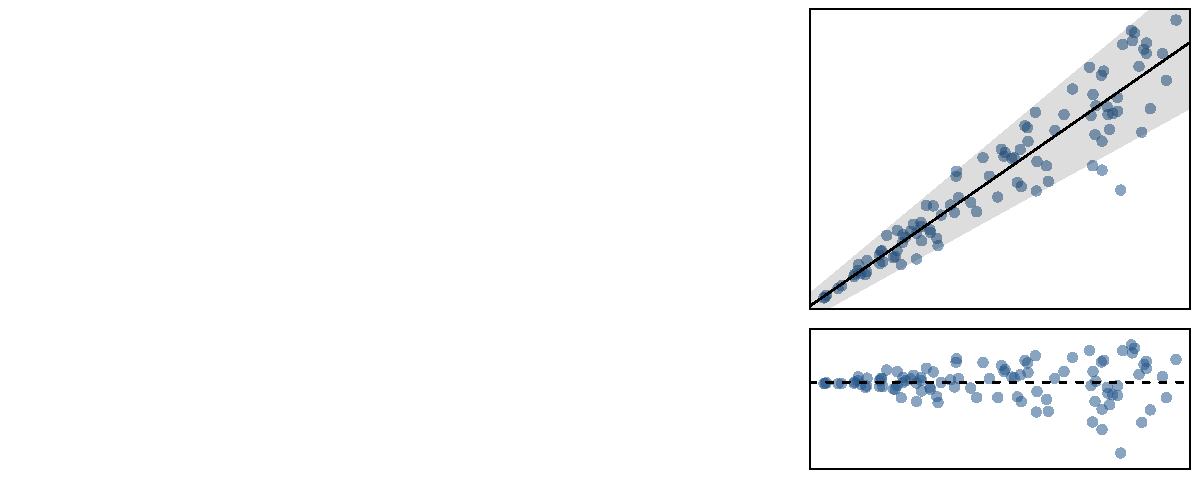
\includegraphics[width=\textwidth]{7-2_least_square_reg/figures/problems/heteroscedastic}
\end{center}
}

\end{frame}

%%%%%%%%%%%%%%%%%%%%%%%%%%%%%%%%%%

\subsection{$R^2$}

%%%%%%%%%%%%%%%%%%%%%%%%%%%%%%%%%%%

\begin{frame}
\frametitle{$R^2$}

\begin{itemize}

\item The strength of the fit of a linear model is most commonly evaluated using \mathhl{R^2}.

\pause

\item $R^2$ is calculated as the square of the correlation coefficient.

\pause

\item It tells us what percent of variability in the response variable is explained by the model.

\pause

\item The remainder of the variability is explained by variables not included in the model or by inherent randomness in the data.

\pause

\item For the model we've been working with, $R^2 = -0.62^2 = 0.38$.

\end{itemize}

\end{frame}

%%%%%%%%%%%%%%%%%%%%%%%%%%%%%%%%%%

\begin{frame}
\frametitle{Interpretation of $R^2$}

\pq{{\small Which of the below is the correct interpretation of $R = -0.62$, $R^2 = 0.38$?}}

\twocol{0.65}{0.35}{
\begin{enumerate}[(a)]

\item 38\% of the variability in the \% of HG graduates among the 51 states is explained by the model.

\solnMult{ 38\% of the variability in the \% of residents living in poverty among the 51 states is explained by the model.}

\item 38\% of the time \% HS graduates predict \% living in poverty correctly.

\item 62\% of the variability in the \% of residents living in poverty among the 51 states is explained by the model.

\end{enumerate}
}{
\begin{center}
\includegraphics[width=\textwidth]{7-2_least_square_reg/figures/poverty/poverty_hsgrad}
\end{center}
}

\end{frame}

%%%%%%%%%%%%%%%%%%%%%%%%%%%%%%%%%%

\subsection{Categorical explanatory variables}

%%%%%%%%%%%%%%%%%%%%%%%%%%%%%%%%%%%

\begin{frame}
\frametitle{Poverty vs. region (east, west)}


\[ \widehat{poverty} = 11.17 + 0.38 \times west \]

\begin{itemize}

\item Explanatory variable: region, \hl{reference level:} east

\item \hl{Intercept:} The estimated average poverty percentage in eastern states is 11.17\%
\pause
\begin{itemize}
\item This is the value we get if we plug in \red{0} for the explanatory variable
\end{itemize}

\pause

\item \hl{Slope:} The estimated average poverty percentage in western states is 0.38\% higher than eastern states.
\pause
\begin{itemize}
\item Then, the estimated average poverty percentage in western states is 11.17 + 0.38 =  11.55\%.
\pause
\item This is the value we get if we plug in \red{1} for the explanatory variable
\end{itemize}

\end{itemize}

\end{frame}

%%%%%%%%%%%%%%%%%%%%%%%%%%%%%%%%%%

\begin{frame}
\frametitle{Poverty vs. region (northeast, midwest, west, south)}

\pq{Which region (northeast, midwest, west, or south) is the reference level?}

{\small
\begin{center}
\begin{tabular}{rrrrr}
  \hline
 & Estimate & Std. Error & t value & Pr($>$$|$t$|$) \\ 
  \hline
(Intercept) & 9.50 & 0.87 & 10.94 & 0.00 \\ 
region4midwest & 0.03 & 1.15 & 0.02 & 0.98 \\ 
region4west & 1.79 & 1.13 & 1.59 & 0.12 \\ 
region4south & 4.16 & 1.07 & 3.87 & 0.00 \\ 
   \hline
\end{tabular}
\end{center}
}

\begin{enumerate}[(a)]
\solnMult{northeast}
\item midwest
\item west
\item south
\item cannot tell
\end{enumerate}

\end{frame}

%%%%%%%%%%%%%%%%%%%%%%%%%%%%%%%%%%%

\begin{frame}
\frametitle{Poverty vs. region (northeast, midwest, west, south)}

\pq{Which region (northeast, midwest, west, or south) has the lowest poverty percentage?}

{\small
\begin{center}
\begin{tabular}{rrrrr}
  \hline
 & Estimate & Std. Error & t value & Pr($>$$|$t$|$) \\ 
  \hline
(Intercept) & 9.50 & 0.87 & 10.94 & 0.00 \\ 
region4midwest & 0.03 & 1.15 & 0.02 & 0.98 \\ 
region4west & 1.79 & 1.13 & 1.59 & 0.12 \\ 
region4south & 4.16 & 1.07 & 3.87 & 0.00 \\ 
   \hline
\end{tabular}
\end{center}
}

\begin{enumerate}[(a)]
\solnMult{northeast}
\item midwest
\item west
\item south
\item cannot tell
\end{enumerate}

\end{frame}

%%%%%%%%%%%%%%%%%%%%%%%%%%%%%%%%%%%%

\section{Types of outliers in linear regression}

%%%%%%%%%%%%%%%%%%%%%%%%%%%%%%%%%%%%

\begin{frame}
\frametitle{Types of outliers}

\twocol{0.5}{0.5}
{
\dq{How do outliers influence the least squares line in this plot?}

To answer this question think of where the regression line would be with and without the outlier(s). Without the outliers the regression line would be steeper, and lie closer to the larger group of observations. With the outliers the line is pulled up and away from some of the observations in the larger group. 
}
{
\begin{center}
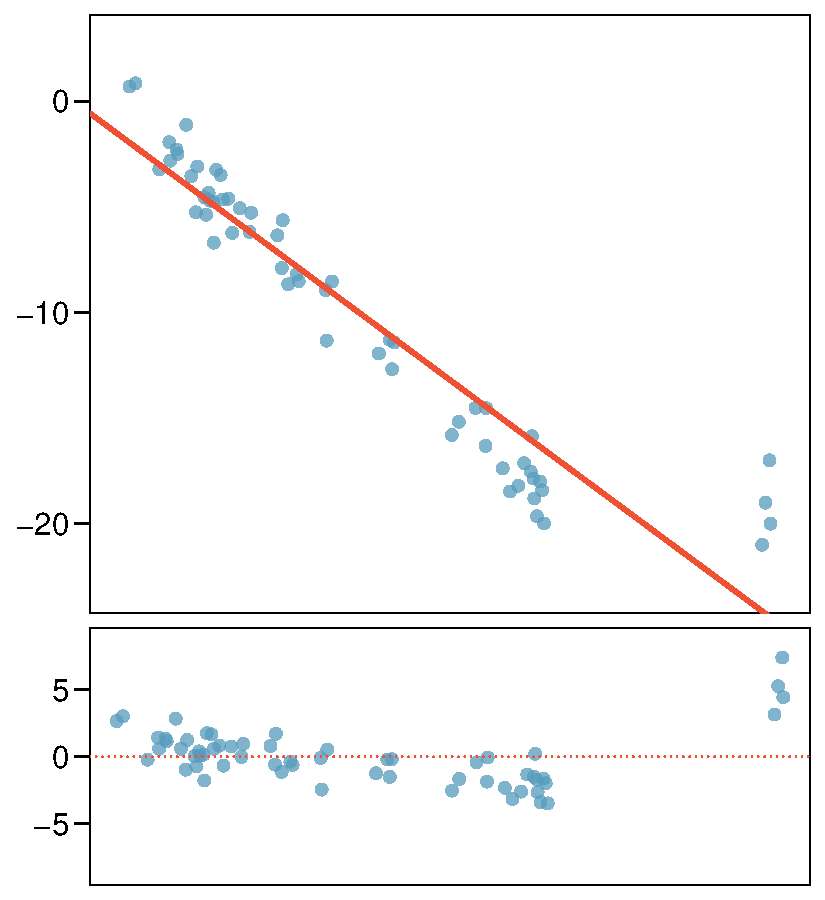
\includegraphics[width=\textwidth]{7-3_outliers/figures/outlierPlots/out4}
\end{center}
}

\end{frame}

%%%%%%%%%%%%%%%%%%%%%%%%%%%%%%%%%%%

\begin{frame}
\frametitle{Types of outliers}

\twocol{0.4}{0.6}
{
\dq{How do outliers influence the least squares line in this plot?} \\
\soln{\only<2>{Without the outlier there is no evident relationship between $x$ and $y$.}}
}
{
\begin{center}
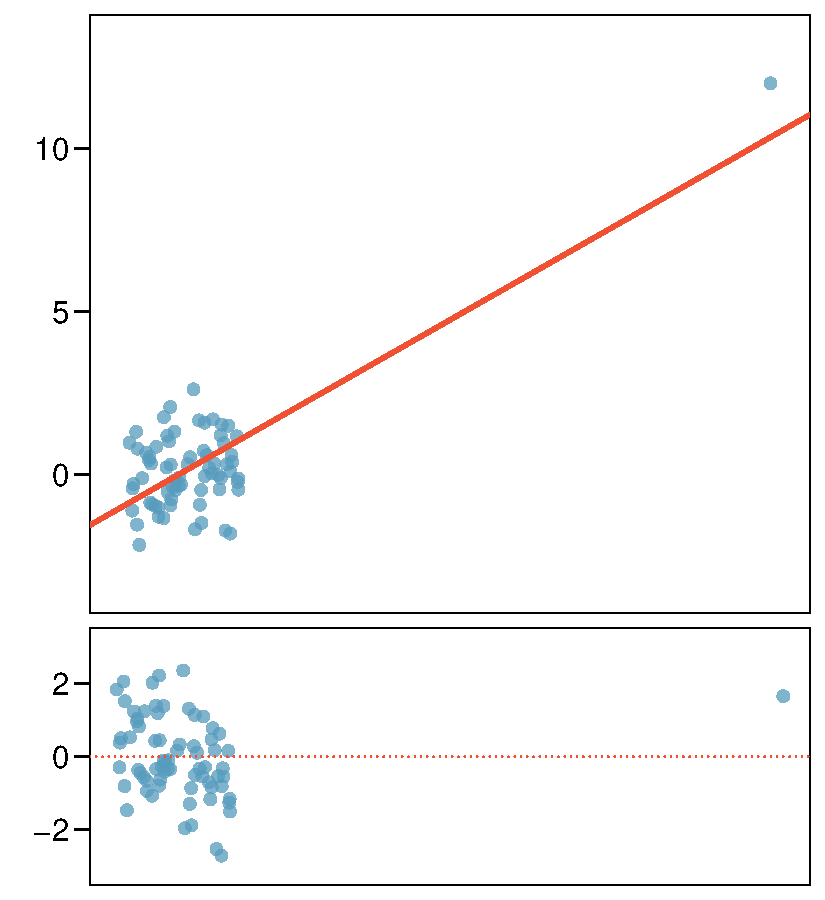
\includegraphics[width=\textwidth]{7-3_outliers/figures/outlierPlots/out5}
\end{center}
}

\end{frame}

%%%%%%%%%%%%%%%%%%%%%%%%%%%%%%%%%%%

\begin{frame}
\frametitle{Some terminology}
 
\begin{itemize}

\item \hl{Outliers} are points that lie away from the cloud  of points.

\pause

\item Outliers that lie horizontally away from the center of the cloud are called \hl{high leverage} points.

\pause

\item High leverage points that actually influence the \underline{slope} of the regression line are called \hl{influential} points.

\pause

\item In order to determine if a point is influential, visualize the regression line with and without the point. Does the slope of the line change considerably? If so, then the point is influential. If not, then it�s not an influential point.

\end{itemize}

\end{frame}

%%%%%%%%%%%%%%%%%%%%%%%%%%%%%%%%%%%

\begin{frame}
\frametitle{Influential points}

Data are available on the log of the surface temperature and the log of the light intensity of 47 stars in the star cluster CYG OB1.

\twocol{0.7}{0.3}
{
\begin{center}
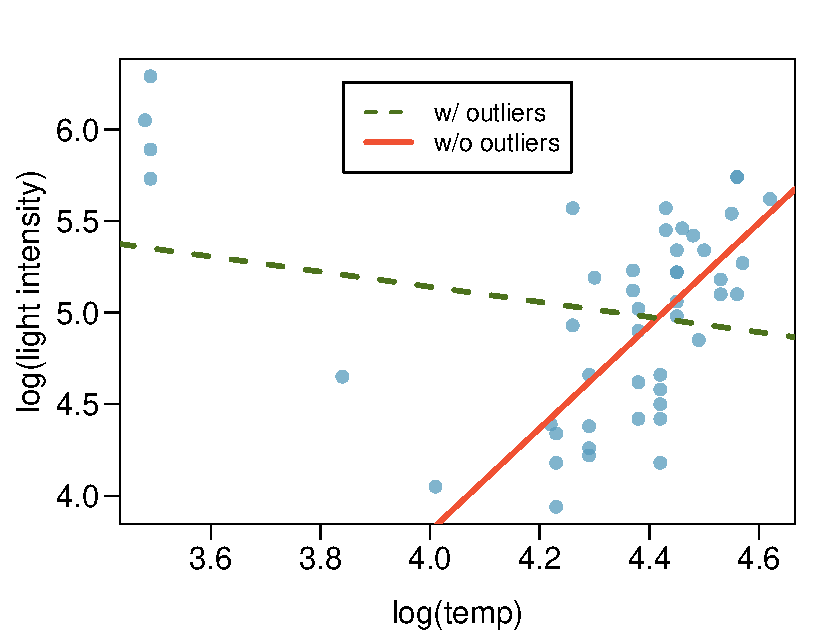
\includegraphics[width=\textwidth]{7-3_outliers/figures/stars/star}
\end{center}
}
{
\begin{center}
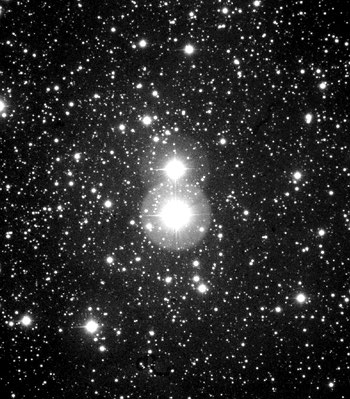
\includegraphics[width=\textwidth]{7-3_outliers/figures/stars/cyg}
\end{center}
}

\end{frame}

%%%%%%%%%%%%%%%%%%%%%%%%%%%%%%%%%%%

\begin{frame}
\frametitle{Types of outliers}

\twocol{0.4}{0.6}
{
\pq{Which of the below best describes the outlier?}
\begin{enumerate}[(a)]
\item influential
\solnMult{high leverage}
\item none of the above
\item there are no outliers
\end{enumerate}
}
{
\begin{center}
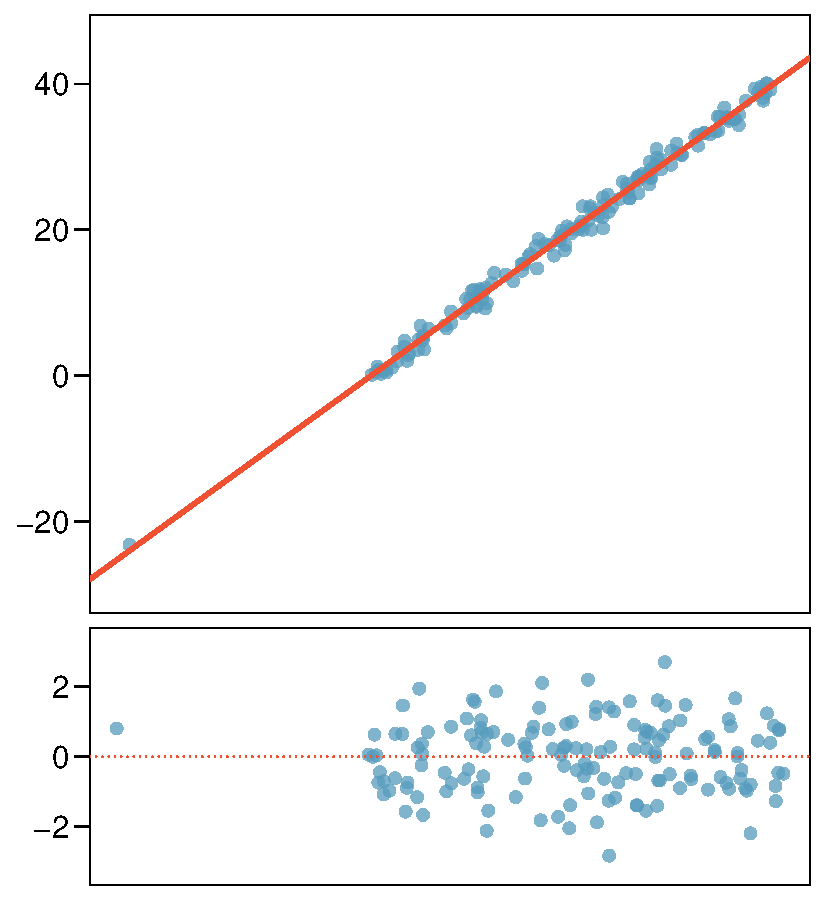
\includegraphics[width=\textwidth]{7-3_outliers/figures/outlierPlots/out6}
\end{center}
}

\end{frame}

%%%%%%%%%%%%%%%%%%%%%%%%%%%%%%%%%%%

\begin{frame}
\frametitle{Types of outliers}

\twocol{0.4}{0.6}
{
\dq{Does this outlier influence the slope of the regression line?}
\soln{\only<2>{Not much...}}

}
{
\begin{center}
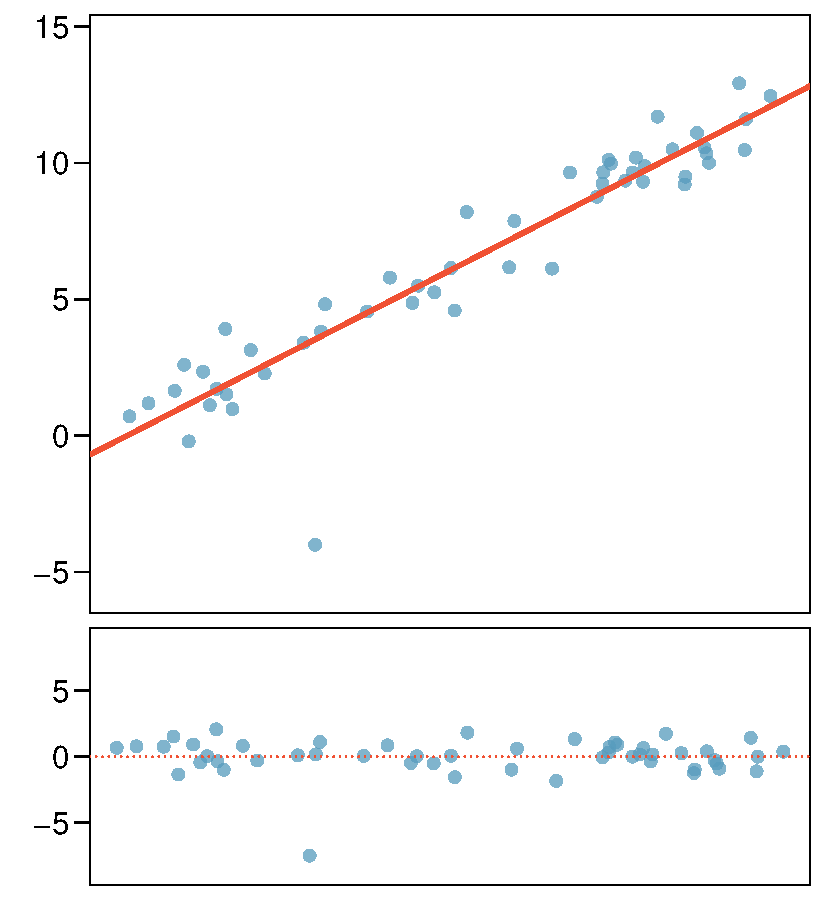
\includegraphics[width=\textwidth]{7-3_outliers/figures/outlierPlots/out1}
\end{center}
}

\end{frame}

%%%%%%%%%%%%%%%%%%%%%%%%%%%%%%%%%%%

\begin{frame}
\frametitle{Recap}

\pq{Which of following is \underline{true}?}

\begin{enumerate}[(a)]
\item Influential points always change the intercept of the regression line.
\item Influential points always reduce $R^2$.
\item It is much more likely for a low leverage point to be influential, than a high leverage point.
\item When the data set includes an influential point, the relationship between the explanatory variable and the response variable is always nonlinear.
\solnMult{None of the above.}
\end{enumerate}

\end{frame}

%%%%%%%%%%%%%%%%%%%%%%%%%%%%%%%%%%%

\begin{frame}
\frametitle{Recap (cont.)}

\vspace{-1cm}

\twocol{0.5}{0.5}
{
\begin{center}
\[ R = 0.08, R^2 = 0.0064 \]
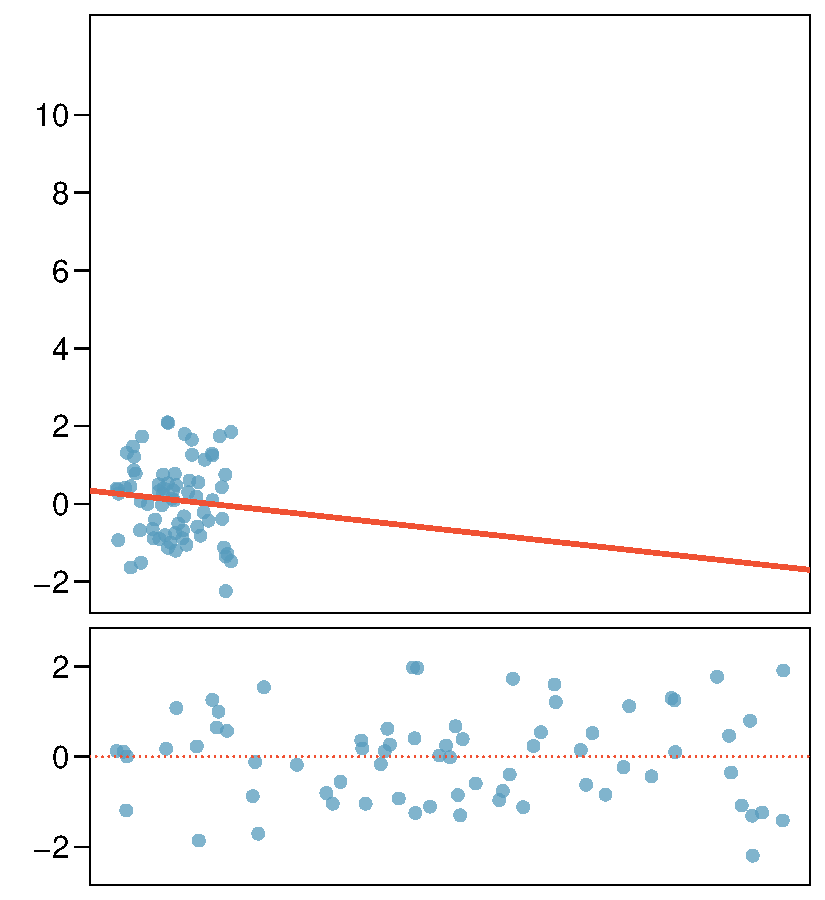
\includegraphics[width=\textwidth]{7-3_outliers/figures/outlierPlots/out5-1}
\end{center}
}
{
\begin{center}
\[ R = 0.79, R^2 = 0.6241 \]
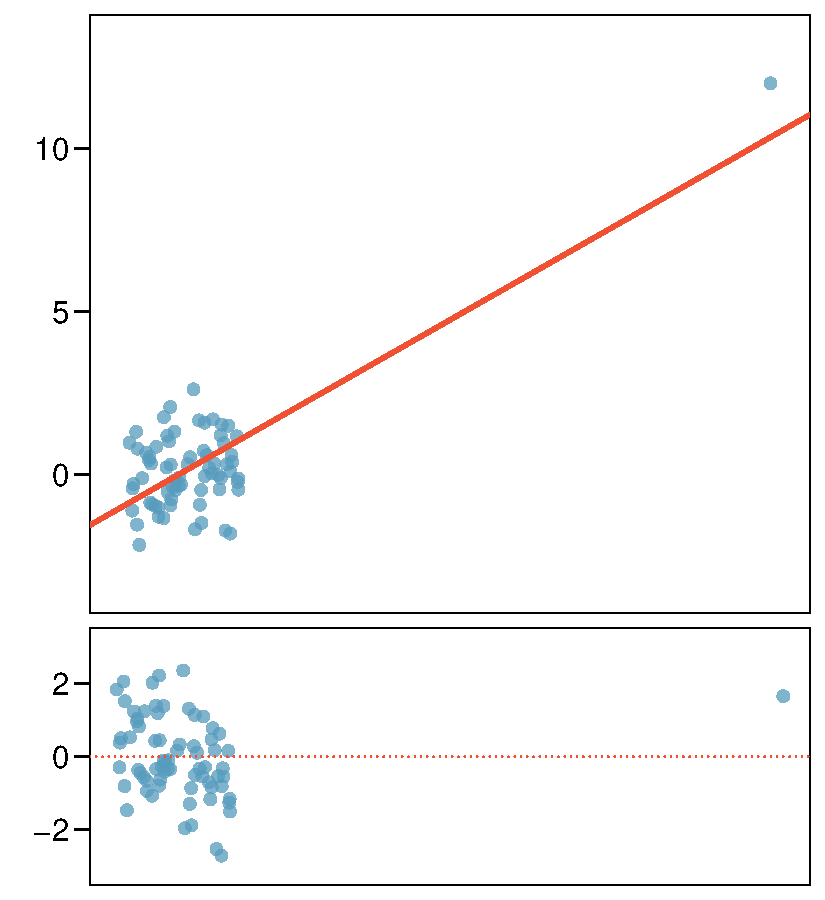
\includegraphics[width=\textwidth]{7-3_outliers/figures/outlierPlots/out5}
\end{center}
}

\end{frame}

\section{Inference for linear regression}

%%%%%%%%%%%%%%%%%%%%%%%%%%%%%%%%%%%%

\subsection{Understanding regression output from software}

%%%%%%%%%%%%%%%%%%%%%%%%%%%%%%%%%%%

\begin{frame}
\frametitle{Nature or nurture?}

{\small In 1966 Cyril Burt published a paper called ``The genetic determination of differences in intelligence: A study of monozygotic twins reared apart?" The data consist of IQ scores for [an assumed random sample of] 27 identical twins, one raised by foster parents, the other by the biological parents.}

\begin{center}
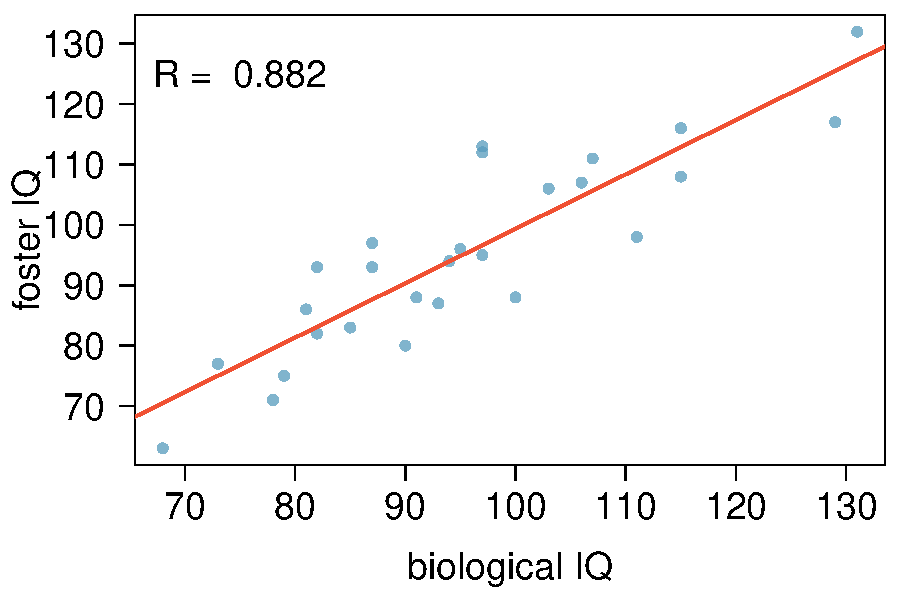
\includegraphics[width=0.7\textwidth]{7-4_inf_lin_reg/figures/twins/twins_IQ}
\end{center}

\end{frame}

%%%%%%%%%%%%%%%%%%%%%%%%%%%%%%%%%%%

\begin{frame}[fragile]
\frametitle{}

\pq{Which of the following is \underline{false}?}

{\footnotesize
\begin{verbatim}
Coefficients:
                 Estimate Std. Error t value Pr(>|t|)    
(Intercept)       9.20760    9.29990   0.990    0.332    
bioIQ             0.90144    0.09633   9.358  1.2e-09

Residual standard error: 7.729 on 25 degrees of freedom
Multiple R-squared: 0.7779,	Adjusted R-squared: 0.769 
F-statistic: 87.56 on 1 and 25 DF,  p-value: 1.204e-09 
\end{verbatim}
}

\begin{enumerate}[(a)]
\item Additional 10 points in the biological twin's IQ is associated with additional 9 points in the foster twin's IQ, on average.
\solnMult{Roughly 78\% of the foster twins' IQs can be accurately predicted by the model.}
\item The linear model is $\widehat{fosterIQ} = 9.2 + 0.9 \times bioIQ$.
\item Foster twins with IQs higher than average IQs tend to have biological twins with higher than average IQs as well.
\end{enumerate}

\end{frame}

%%%%%%%%%%%%%%%%%%%%%%%%%%%%%%%%%%%

\subsection{HT for the slope}

%%%%%%%%%%%%%%%%%%%%%%%%%%%%%%%%%%%

\begin{frame}
\frametitle{Testing for the slope}

\pq{Assuming that these 27 twins comprise a representative sample of all twins separated at birth, we would like to test if these data provide convincing evidence that the IQ of the biological twin is a significant predictor of IQ of the foster twin. What are the appropriate hypotheses?}

\begin{enumerate}[(a)]
\item \mathhl{H_0:} $b_0 = 0$; \mathhl{H_A:} $b_0 \ne 0$ 
\item \mathhl{H_0:} $\beta_0 = 0$; \mathhl{H_A:} $\beta_0 \ne 0$ 
\item \mathhl{H_0:} $b_1 = 0$; \mathhl{H_A:} $b_1 \ne 0$ 
\solnMult{ \mathhl{H_0:} $\beta_1 = 0$; \mathhl{H_A:} $\beta_1 \ne 0$ }
\end{enumerate}

\end{frame}

%%%%%%%%%%%%%%%%%%%%%%%%%%%%%%%%%%%

\begin{frame}
\frametitle{Testing for the slope (cont.)}

{\footnotesize
\begin{center}
\begin{tabular}{rrrrr}
  \hline
 & Estimate & Std. Error & t value & Pr($>$$|$t$|$) \\ 
  \hline
(Intercept) & 9.2076 & 9.2999 & 0.99 & 0.3316 \\ 
  bioIQ & 0.9014 & 0.0963 & 9.36 & 0.0000 \\ 
   \hline
\end{tabular}
\end{center}
}

\pause

\begin{itemize}

\item We always use a $t$-test in inference for regression. $\:$ \\

\pause

\Remember{Test statistic, $T = \frac{point~estimate - null~value}{SE}$}

\pause

\item Point estimate = $b_1$ is the observed slope.

\pause

\item $SE_{b_1}$ is the standard error associated with the slope.

\pause

\item Degrees of freedom associated with the slope is $df = n - 2$, where $n$ is the sample size. $\:$ \\
\pause
\Remember{We lose 1 degree of freedom for each parameter we estimate, and in simple linear regression we estimate 2 parameters, $\beta_0$ and $\beta_1$.}

\end{itemize}

\end{frame}

%%%%%%%%%%%%%%%%%%%%%%%%%%%%%%%%%%%

\begin{frame}
\frametitle{Testing for the slope (cont.)}

{\small
\begin{center}
\begin{tabular}{rrrrr}
  \hline
 & Estimate & Std. Error & t value & Pr($>$$|$t$|$) \\ 
  \hline
(Intercept) &  9.2076 & 9.2999 & 0.99 & 0.3316 \\ 
  bioIQ & \red{0.9014}  &   \green{0.0963} & \orange{9.36} & \textcolor{blue}{0.0000} \\ 
   \hline
\end{tabular}
\end{center}
}

\pause

\begin{eqnarray*}
T &=& \frac{\red{0.9014} - 0}{\green{0.0963}} = \orange{9.36} \\
\pause
df &=& 27 - 2 = 25 \\
\pause
p-value &=& P(|T| > \orange{9.36}) < \textcolor{blue}{0.01}
\end{eqnarray*}

\end{frame}

%%%%%%%%%%%%%%%%%%%%%%%%%%%%%%%%%%%

\begin{frame}
\frametitle{\% College graduate vs. \% Hispanic in LA}

\dq{What can you say about the relationship between \% college graduate and \% Hispanic in a sample of 100 zip code areas in LA?}

\begin{center}
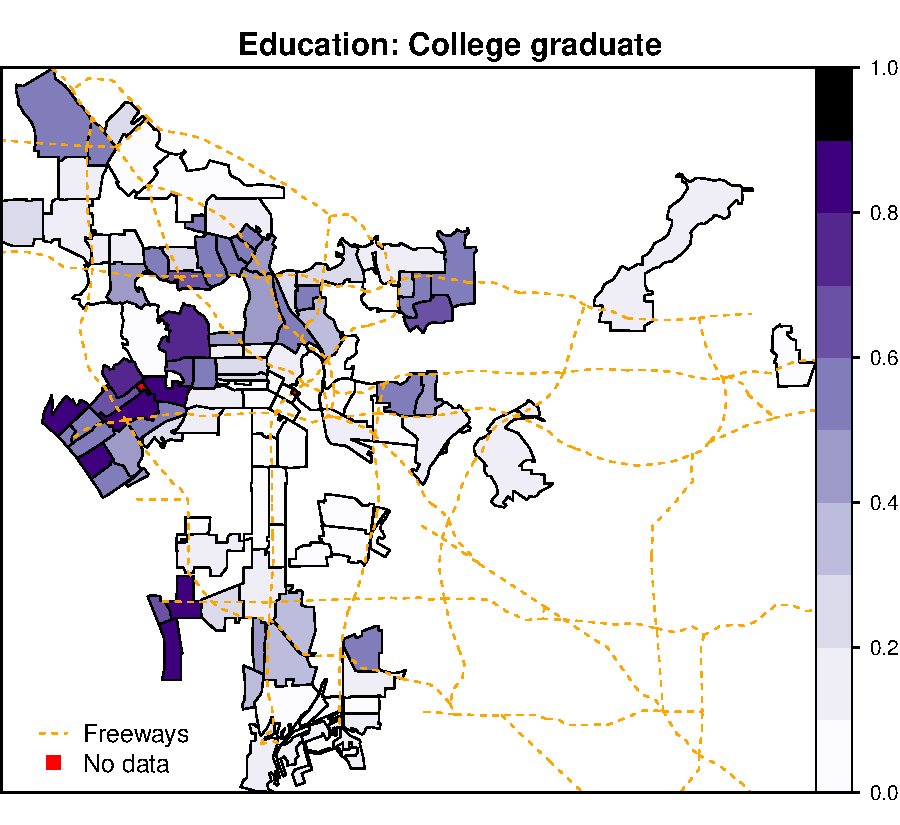
\includegraphics[width=0.53\textwidth]{7-4_inf_lin_reg/figures/la/Prop_EduHigherThan16th}
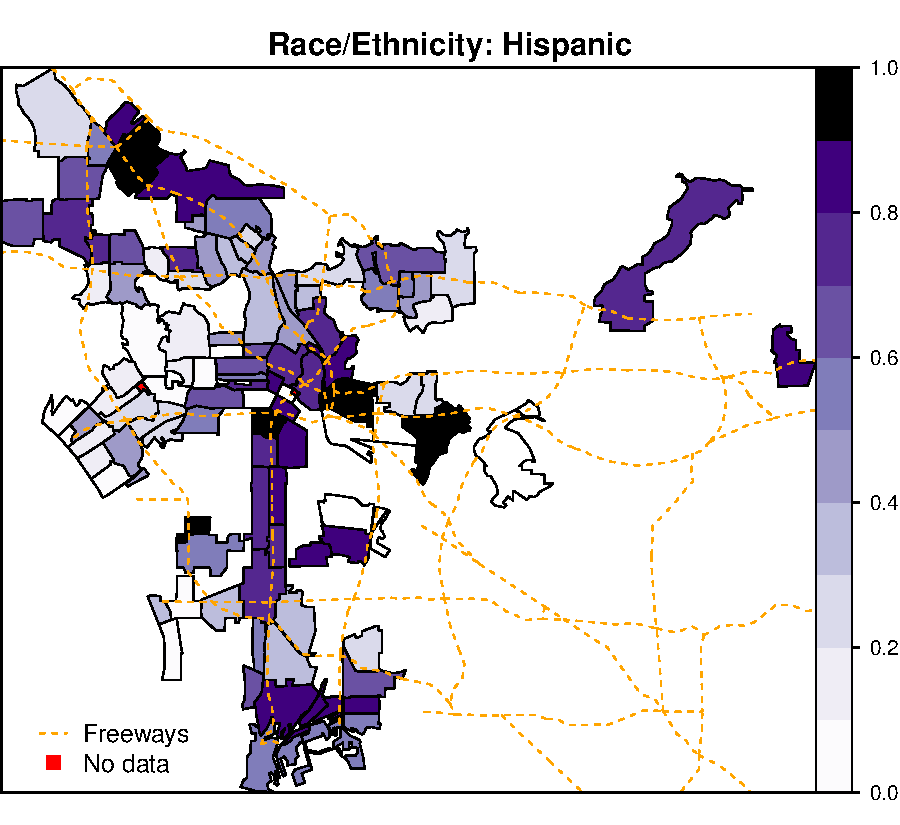
\includegraphics[width=0.53\textwidth]{7-4_inf_lin_reg/figures/la/Prop_RaceEthHispanic}
\end{center}

\end{frame}

%%%%%%%%%%%%%%%%%%%%%%%%%%%%%%%%%%%

\begin{frame}
\frametitle{\% College educated vs. \% Hispanic in LA - another look}

\dq{What can you say about the relationship between of \% college graduate and \% Hispanic in a sample of 100 zip code areas in LA?}

\begin{center}
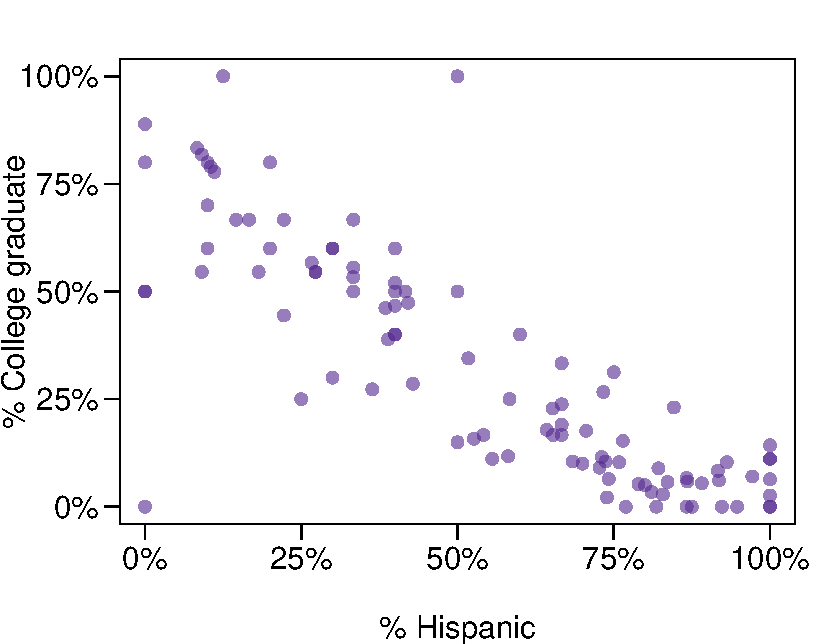
\includegraphics[width=0.7\textwidth]{7-4_inf_lin_reg/figures/la/la}
\end{center}

\end{frame}

%%%%%%%%%%%%%%%%%%%%%%%%%%%%%%%%%%%

\begin{frame}
\frametitle{\% College educated vs. \% Hispanic in LA - linear model}

\pq{Which of the below is the best interpretation of the slope?}

{\small
\begin{center}
\begin{tabular}{rrrrr}
  \hline
 & Estimate & Std. Error & t value & Pr($>$$|$t$|$) \\ 
  \hline
(Intercept) & 0.7290 & 0.0308 & 23.68 & 0.0000 \\ 
 \%Hispanic & -0.7527 & 0.0501 & -15.01 & 0.0000 \\ 
   \hline
%   &&&&$df$ = 98 \\
\end{tabular}
\end{center}
}

\begin{enumerate}[(a)]
\item A 1\% increase in Hispanic residents in a zip code area in LA is associated with a 75\% decrease in \% of college grads.
\solnMult{A 1\% increase in Hispanic residents in a zip code area in LA is associated with a 0.75\% decrease in \% of college grads.}
\item An additional 1\% of Hispanic residents decreases the \% of college graduates in a zip code area in LA by 0.75\%.
\item In zip code areas with no Hispanic residents, \% of college graduates is expected to be 75\%.
\end{enumerate}

\end{frame}

%%%%%%%%%%%%%%%%%%%%%%%%%%%%%%%%%%%

\begin{frame}
\frametitle{\% College educated vs. \% Hispanic in LA - linear model}

\dq{Do these data provide convincing evidence that there is a statistically significant relationship between \% Hispanic and \% college graduates in zip code areas in LA?}

{\small
\begin{center}
\begin{tabular}{rrrrr}
  \hline
 & Estimate & Std. Error & t value & Pr($>$$|$t$|$) \\ 
  \hline
(Intercept) & 0.7290 & 0.0308 & 23.68 & 0.0000 \\ 
  hispanic & -0.7527 & 0.0501 & -15.01 & 0.0000 \\ 
   \hline
%   &&&&$df$ = 98 \\
\end{tabular}
\end{center}
}
\soln{\only<2->{Yes, the p-value for \% Hispanic is low, indicating that the data provide convincing evidence that the slope parameter is different than 0.
}}

$\:$ \\

\dq{How reliable is this p-value if these zip code areas are not randomly selected?}
\soln{\only<3->{Not very...
}}

\end{frame}

%%%%%%%%%%%%%%%%%%%%%%%%%%%%%%%%%%%

\subsection{CI for the slope}

%%%%%%%%%%%%%%%%%%%%%%%%%%%%%%%%%%%

\begin{frame}
\frametitle{Confidence interval for the slope}

\pq{{\small Remember that a confidence interval is calculated as $point~estimate \pm ME$ and the degrees of freedom associated with the slope in a simple linear regression is $n - 2$. Which of the below is the correct 95\% confidence interval for the slope parameter? Note that the model is based on observations from 27 twins.}}

{\footnotesize
\begin{center}
\begin{tabular}{rrrrr}
  \hline
 & Estimate & Std. Error & t value & Pr($>$$|$t$|$) \\ 
  \hline
(Intercept) & 9.2076 & 9.2999 & 0.99 & 0.3316 \\ 
  bioIQ & 0.9014 & 0.0963 & 9.36 & 0.0000 \\ 
   \hline
\end{tabular}
\end{center}
}

\vspace{-0.5cm}

\twocol{0.4}{0.6}
{
\begin{enumerate}[(a)]
\item $9.2076 \pm 1.65 \times 9.2999$
\solnMult{ $0.9014 \pm 2.06 \times 0.0963$}
\item $0.9014 \pm 1.96 \times 0.0963$
\item $9.2076 \pm 1.96 \times 0.0963$
\end{enumerate}
}
{
\soln{\onslide<2->{\red{
\begin{eqnarray*}
\pause
n &=& 27 \qquad df = 27 - 2 = 25 \\
\pause
95\%:~t^\star_{25} &=& 2.06 \\
\pause
0.9014 &\pm& 2.06 \times 0.0963 \\
\pause
(0.7 &,& 1.1)
\end{eqnarray*}
}}}}

\end{frame}

%%%%%%%%%%%%%%%%%%%%%%%%%%%%%%%%%%%

\begin{frame}
\frametitle{Recap}

\begin{itemize}

\item Inference for the slope for a single-predictor linear regression model:
\pause
\begin{itemize}
\item Hypothesis test:
\[ T = \frac{b_1 - null~value}{SE_{b_1}} \qquad df = n - 2 \]
\pause
\item Confidence interval:
\[ b_1 \pm t^\star_{df = n - 2} SE_{b_1} \]
\end{itemize}

\pause

\item The null value is often 0 since we are usually checking for \hl{any} relationship between the explanatory and the response variable.

\pause

\item The regression output gives $b_1$, $SE_{b_1}$, and \hl{two-tailed} p-value for the $t$-test for the slope where the null value is 0.

\pause

\item We rarely do inference on the intercept, so we'll be focusing on the estimates and inference for the slope.

\end{itemize}

\end{frame}

%%%%%%%%%%%%%%%%%%%%%%%%%%%%%%%%%%%


\begin{frame}
\frametitle{Caution}

\begin{itemize}

\item Always be aware of the type of data you're working with: random sample, non-random sample, or population.

\pause

\item Statistical inference, and the resulting p-values, are meaningless when you already have population data.

\pause

\item If you have a sample that is non-random (biased), inference on the results will be unreliable.

\pause

\item The ultimate goal is to have independent observations.

\end{itemize}

\end{frame}

%%%%%%%%%%%%%%%%%%%%%%%%%%%%%%%%%%%


%%%%%%%%%%%%%%%%%%%%%%%%%%%%%%%%%%%%

\end{document}